\chapter{Experimental Results}
\label{ch:results}

The V1 tests cover USB-C output regulation, load removal, switching behavior,
input power, and heating. Later V2 tests examine the modified resonant tank
and loading at the secondary output. AC-supply and electronic-load readings
are combined with thermal-region temperatures to describe the higher-load
behavior and the changes still needed for sustained operation.

\section{Tested Prototype and Main Result}
\label{sec:res-bringup}

The highest output calculated from DC-coupled connector voltage and load
current was \SI{79.89}{\watt}. The prototype was also tested at the
\SI{5}{\volt}, \SI{9}{\volt}, \SI{15}{\volt}, and \SI{20}{\volt}
fixed settings with a \SI{240}{\volt}, \SI{50}{\hertz} input. Output voltage was
regulated at the tested loads. A continuous-power rating still needs a
defined-duration test at thermal equilibrium.

The high-load test used an earlier firmware revision; several intermediate-
voltage tests did not record the firmware version. Table~\ref{tab:prototype-identity}
lists the hardware and firmware used in the tests, and
\cref{sec:ctrl-firmware-identities} describes the development stages.

\begin{table}[htbp]
\centering
\caption{Test hardware and firmware.}
\label{tab:prototype-identity}
\begin{tabularx}{\textwidth}{@{}L{0.28\textwidth}X@{}}
\toprule
Item & Test configuration\\
\midrule
Manufactured board & V1.0 PCB with rework; V1.1 documents the corrected circuit\\
Power stage & LMG2652RFBR GaN half bridge; nominal \SI{1}{\mega\hertz} carrier and charge-pump resonant stage\\
Resonant inductance & Two 7443640470B \SI{4.7}{\micro\henry} inductors in series\\
Output interface & MPQ4242GVE-0000-AEC1-P and USB-C connector\\
Controller & STM32G071RBT6; PA8/PA9 carrier, PA10 burst enable, and PA0/PA1/PA2 ADC acquisition\\
Firmware & PWR-1.9.20 in the identified final \SI{5}{\volt} and \SI{20}{\volt} records; unspecified in several \SI{9}{\volt} and \SI{15}{\volt} records; PWR-1.9.10 in the \SI{4.7}{\ampere} high-load record\\
Input & AC source at \SI{240}{\volt}, \SI{50}{\hertz}\\
\bottomrule
\end{tabularx}
\end{table}

Calculations use completed measurements from the load tests. The complete
results are included in the appendix.

DC-coupled captures give mean output voltage, while AC-coupled captures
show small-signal detail and acquisition statistics. Thermal images show
surface hotspots. Error bars are omitted because the uncertainty data are
incomplete; instrument disagreements and ambiguous measurement fields are
discussed with the affected results.

\section{Startup and Shutdown}
\label{sec:res-startup}

The converter reached regulation at all four tested settings. The available
captures begin after startup and lack synchronized command, burst-enable
PA10, output-voltage, and firmware-state traces. Startup delay, inrush,
overshoot, shutdown delay, and discharge time therefore remain unquantified.
The implemented sequences are described in Chapter~\ref{ch:control}.

\section{Steady-State Output Regulation}
\label{sec:res-steady}

The selected average output was maintained through the loaded sweep: up to
\SI{3}{\ampere} at \SI{5}{\volt}, \SI{9}{\volt}, and
\SI{15}{\volt}, and up to \SI{4}{\ampere} at \SI{20}{\volt}.
Average-voltage error was calculated as
\begin{equation}
e_V=\frac{V_\mathrm{BUS,avg}-V_\mathrm{set}}{V_\mathrm{set}}\,100\%,
\label{eq:steady-voltage-error}
\end{equation}
where \(V_\mathrm{BUS,avg}\) is the mean USB-C output voltage. The MCU
regulates the secondary bulk supply feeding the USB-C PD stage.

\begin{figure}[htbp]
\centering
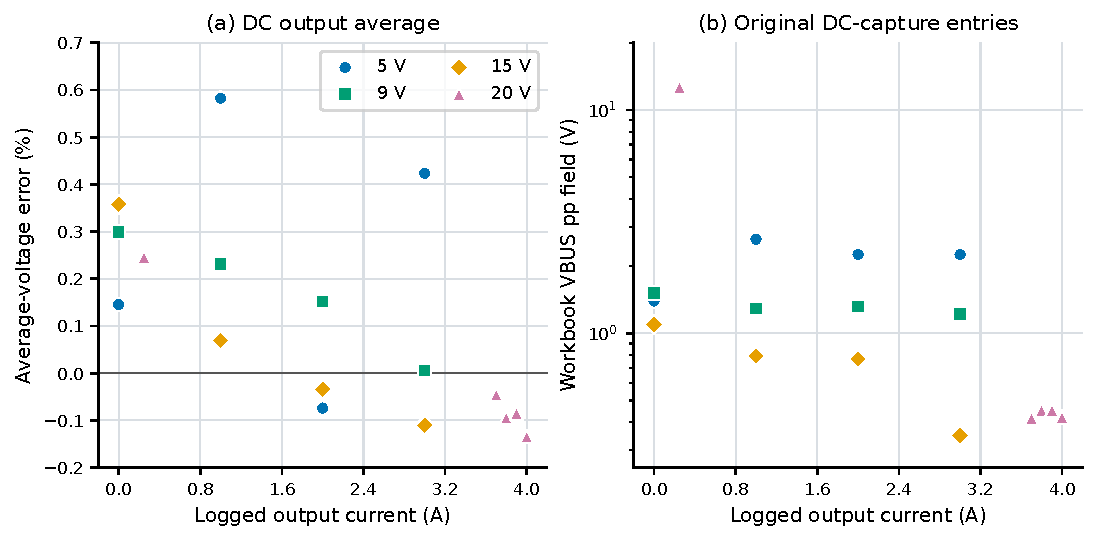
\includegraphics[width=\textwidth]{Pictures/Thesis/10_Results/Rebuilt/regulation_and_logged_ripple.pdf}
\caption{Measured output-voltage error and the workbook VBUS peak-to-peak readings. The right panel uses a logarithmic scale and includes the anomalous workbook values. AC-coupled statistics are plotted separately.}
\label{fig:rebuilt-regulation}
\end{figure}

The largest absolute loaded error was \SI{0.583}{\percent}, at
\SI{5}{\volt} and \SI{1}{\ampere}, with average VBUS of
\SI{5.02913}{\volt}. At maximum load for each lower-voltage setting, the
averages were \SI{5.02118}{\volt}, \SI{9.00057}{\volt}, and
\SI{14.9835}{\volt}. These averages show that the USB-C PD output remained close to its selected
voltage; ripple and transient limits require separate measurements.

\begin{table}[htbp]
\centering
\caption{Maximum-load and high-power measurements. Output power is calculated from average VBUS and load current. The pp column contains the original workbook readings.}
\label{tab:steady-state-results}
\small
\begin{tabular}{@{}rrrrrr@{}}
\toprule
Setting (V) & Load (A) & VBUS avg (V) & Error (\%) & Logged pp (V) & Output (W)\\
\midrule
5 & 3.0 & 5.02118 & +0.424 & 2.252 & 15.06\\
9 & 3.0 & 9.00057 & +0.006 & 1.220 & 27.00\\
15 & 3.0 & 14.98350 & $-0.110$ & 0.349 & 44.95\\
20 & 3.7 & 19.99090 & $-0.046$ & 0.416 & 73.97\\
20 & 3.8 & 19.98130 & $-0.094$ & 0.452 & 75.93\\
20 & 3.9 & 19.98320 & $-0.084$ & 0.453 & 77.93\\
20 & 4.0 & 19.97320 & $-0.134$ & 0.421 & 79.89\\
\bottomrule
\end{tabular}
\end{table}

At \SI{20}{\volt}, increasing load from \SI{3.7}{\ampere} to
\SI{4.0}{\ampere} reduced average VBUS by only \SI{17.7}{\milli\volt}
while calculated output rose from \SI{73.97}{\watt} to
\SI{79.89}{\watt}. The \SI{3.8}{\ampere} point exceeded \SI{75}{\watt} calculated output.

\begin{figure}[htbp]
\centering
\begin{subfigure}[t]{0.48\textwidth}
\centering
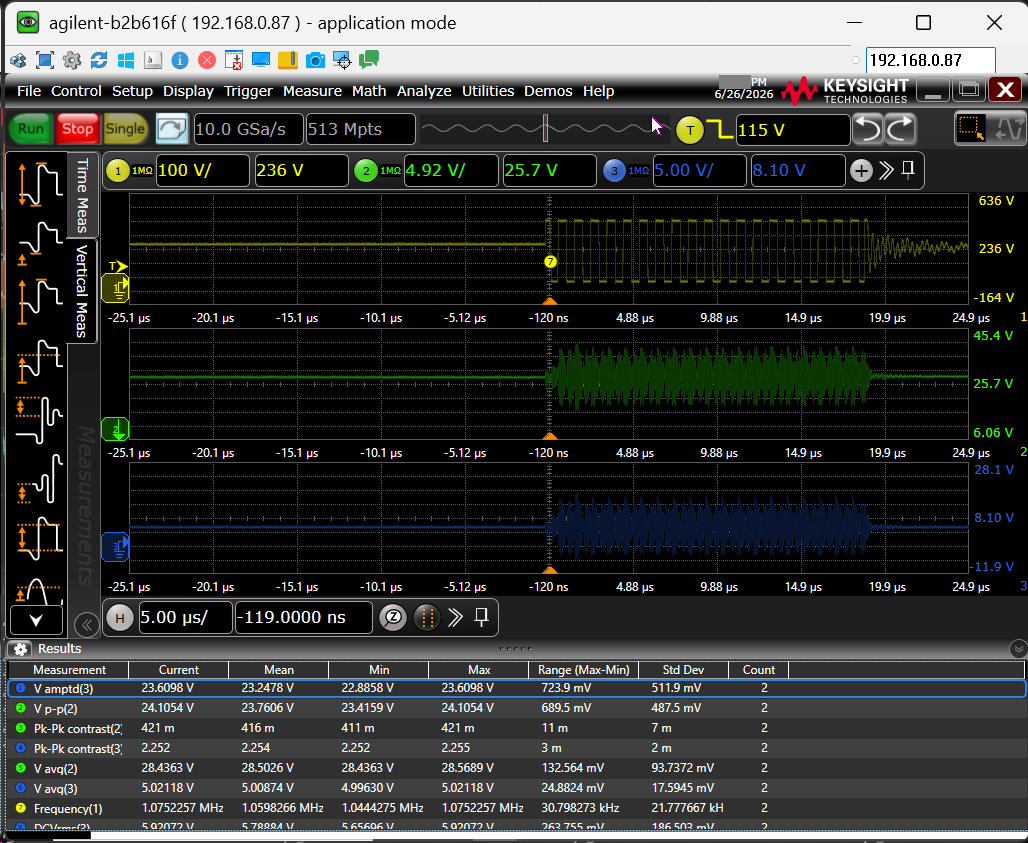
\includegraphics[width=\linewidth]{Data/measurements/evidence/PDO5_15W_3A/keysight_5v_3a_sw_secondary_vbus.png}
\caption{\SI{5}{\volt}, \SI{3}{\ampere}; \sourcefile{PDO5-MAX3A-001}.}
\end{subfigure}\hfill
\begin{subfigure}[t]{0.48\textwidth}
\centering
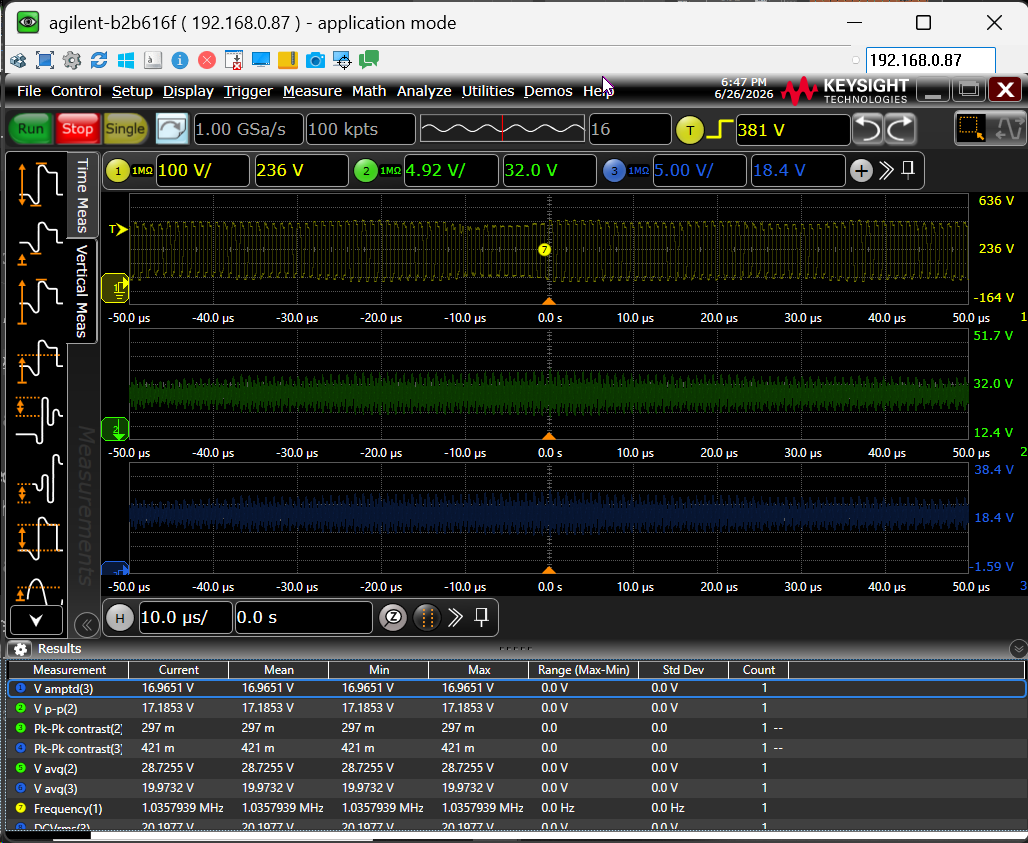
\includegraphics[width=\linewidth]{Data/measurements/evidence/PDO20_80W_40A/keysight_sw_secondary_vbus_20v_40a.png}
\caption{\SI{20}{\volt}, \SI{4}{\ampere}; \sourcefile{PDO20-80W-40A-001}.}
\end{subfigure}
\caption{DC-coupled voltage captures. Yellow: half-bridge switch-node voltage. Green: secondary output voltage. Blue: USB-C VBUS output voltage.}
\label{fig:pdo5-load-sweep-scope}
\label{fig:pdo20-high-power-scope}
\end{figure}

Long-window ripple fields remain unresolved. At \SI{20}{\volt} and
\SI{0.25}{\ampere}, VBUS is listed as \SI{12.6564}{\volt}
``amplitude/ripple.'' Several other pp entries are anomalously large.
The probe, selected measurement, and acquisition window were not fully
recorded, so these values cannot be corrected reliably and must be remeasured.

\subsection{AC-coupled detail captures}

\begin{figure}[htbp]
\centering
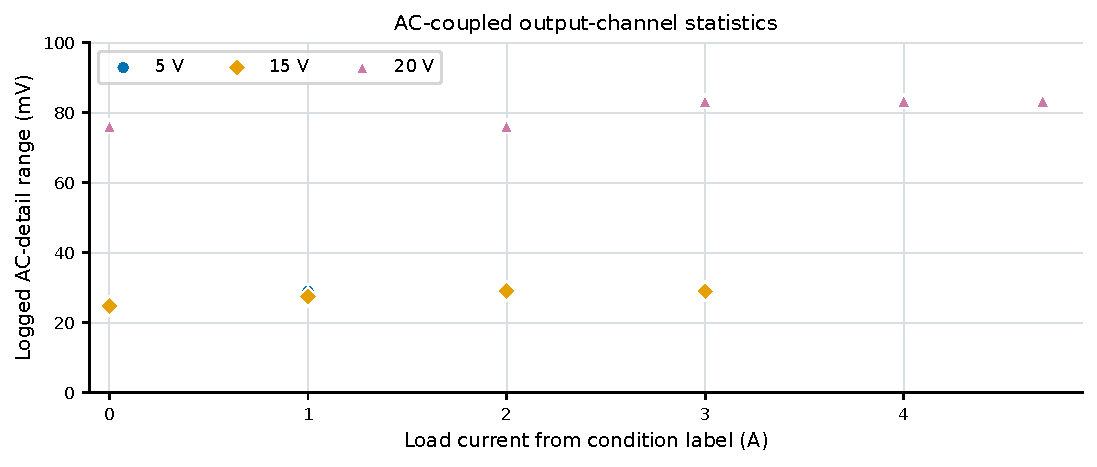
\includegraphics[width=0.95\textwidth]{Pictures/Thesis/10_Results/Rebuilt/ac_detail_statistics.pdf}
\caption{Output-channel statistics from the AC-coupled captures. Several readings are the range of average voltage across acquisitions, rather than instantaneous peak-to-peak ripple.}
\label{fig:rebuilt-ac-detail}
\end{figure}

The later AC-coupled captures used a different probe setup and report VBUS
detail fields of approximately \SI{25}{\milli\volt} to \SI{83}{\milli\volt}.
Several fields are the acquisition-to-acquisition \emph{Range (Max--Min)} of
\emph{V avg}. At \SI{5}{\volt}, \SI{3}{\ampere}, the reported
\SI{29.6924}{\milli\volt} is this statistical spread, rather than
\SI{29.7}{\milli\volt} instantaneous peak-to-peak ripple.

\begin{figure}[htbp]
\centering
\begin{subfigure}[t]{0.48\textwidth}
\centering
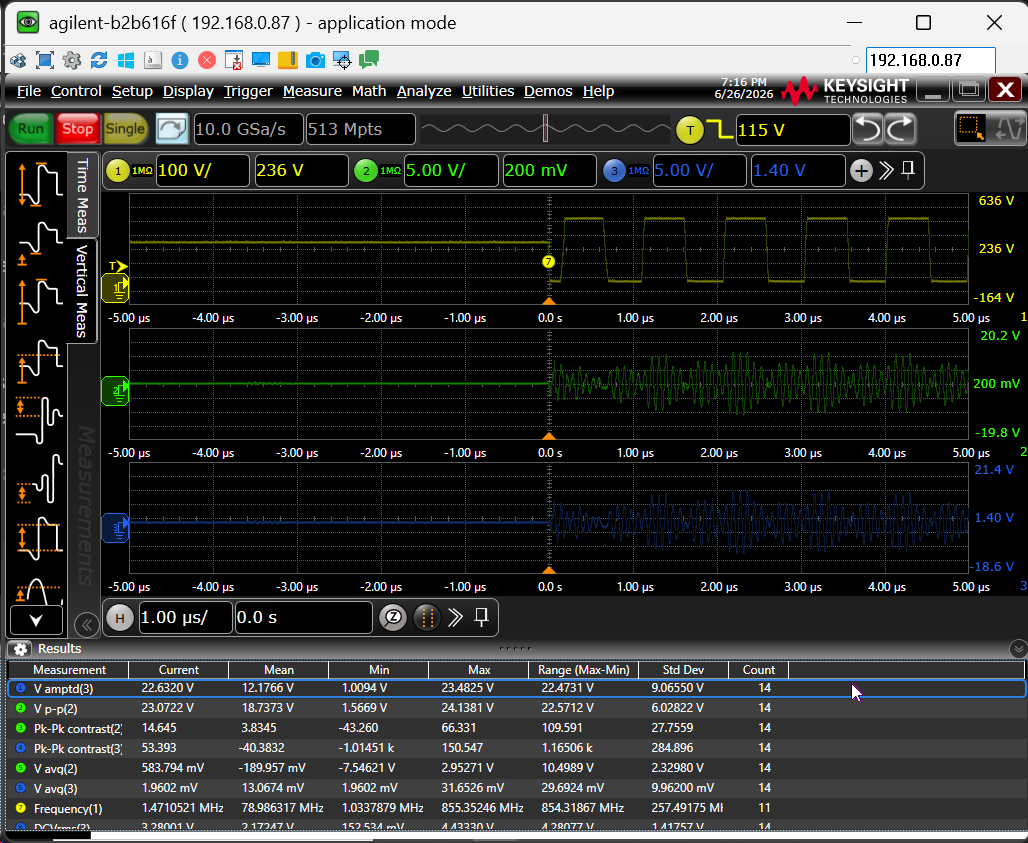
\includegraphics[width=\linewidth]{Data/measurements/evidence/PDO5_15W_3A_AC/keysight_5v_3a_ac_coupled_secondary_vbus.png}
\caption{\SI{5}{\volt}, \SI{3}{\ampere}; range of VBUS-average statistics visible.}
\end{subfigure}\hfill
\begin{subfigure}[t]{0.48\textwidth}
\centering
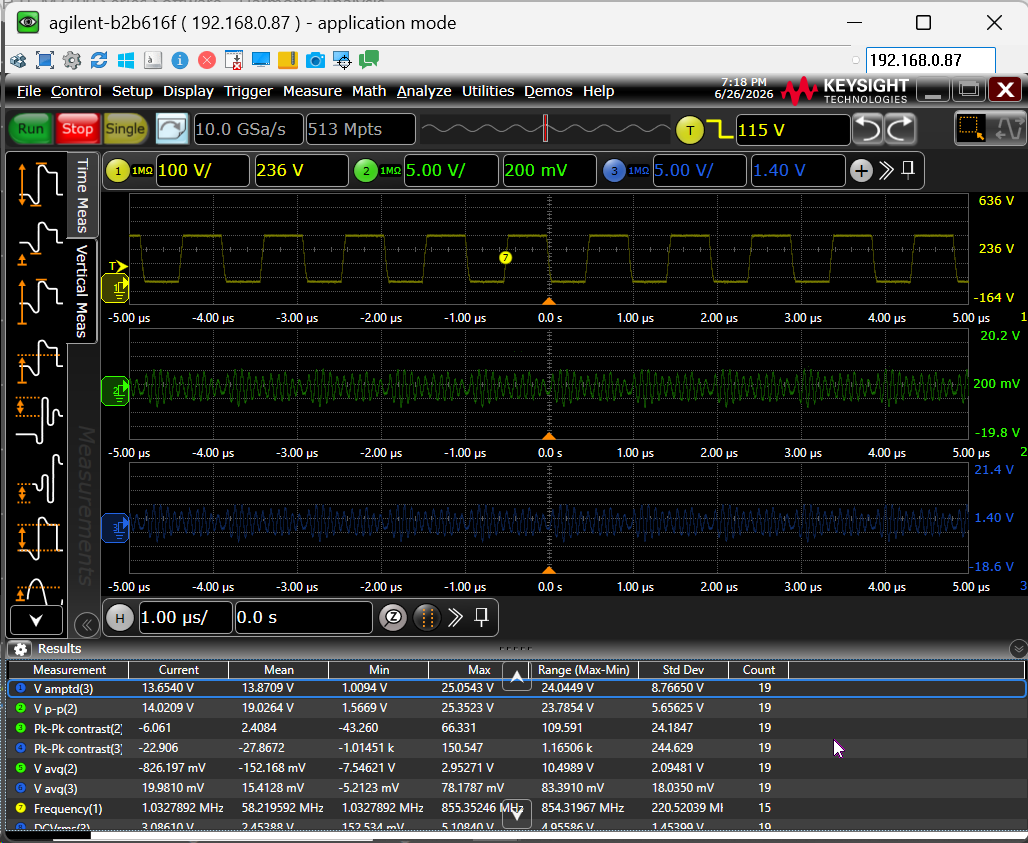
\includegraphics[width=\linewidth]{Data/measurements/evidence/PDO20_80W_4A_AC/keysight_20v_4a_ac_coupled_secondary_vbus.png}
\caption{\SI{20}{\volt}, \SI{4}{\ampere}; AC-coupled output detail.}
\end{subfigure}
\caption{Output ripple captures. Yellow: half-bridge switch-node voltage. Green: secondary output voltage. Blue: USB-C VBUS output voltage. The yellow trace is DC-coupled; the green and blue traces are AC-coupled and show voltage ripple.}
\label{fig:ac-coupled-ripple-scope}
\end{figure}

Table~\ref{tab:ac-coupled-ripple-captures-complete} includes all twelve
detail captures and their source rows. The \SI{20}{\volt},
\SI{4.7}{\ampere} entry has a nominal \SI{94}{\watt} label but no
matching DC output voltage for calculating delivered power. There is also
no completed \SI{20}{\volt}, \SI{4.5}{\ampere} test. The
\SI{20}{\volt} no-load row was excluded from the DC results because its
status is still \emph{Planned}.

\section{Load-Transient Response}
\label{sec:res-transient}

Load-removal tests examined secondary-bus charging by residual resonant
energy. The four captures below show switching and output-voltage response
around disconnection.

\begin{figure}[htbp]
\centering
\begin{subfigure}[t]{0.48\textwidth}
\centering
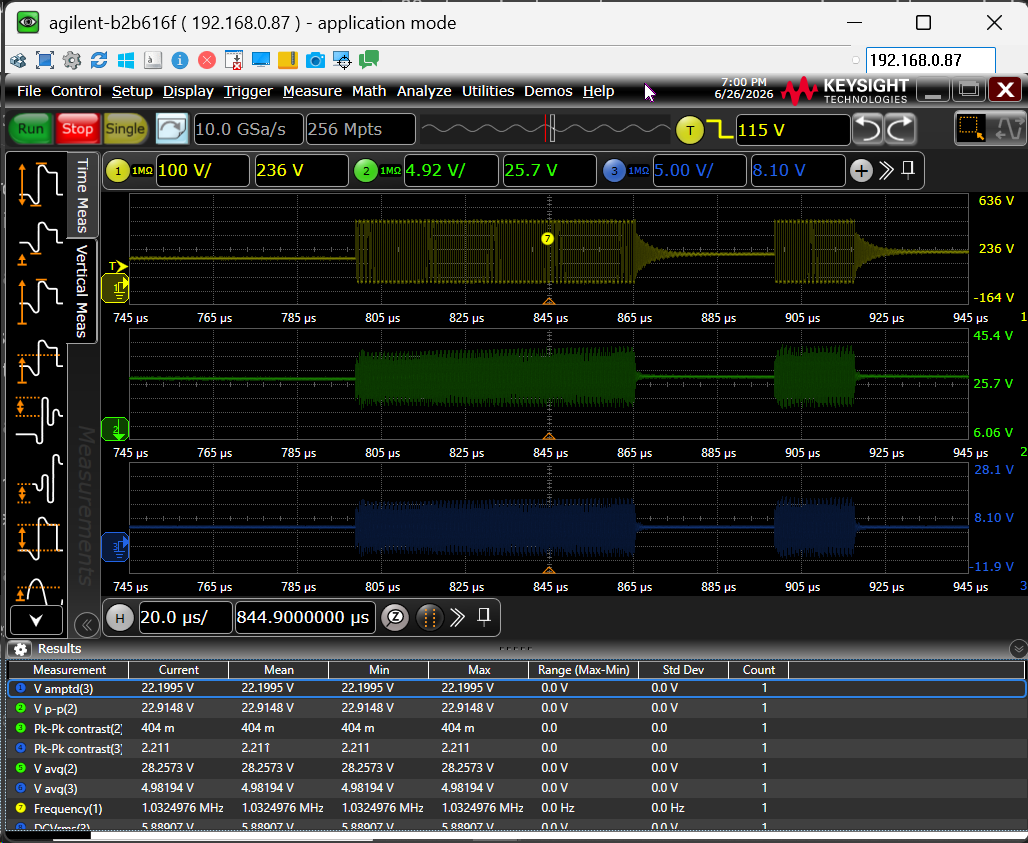
\includegraphics[width=\linewidth]{Data/measurements/evidence/PDO5_3A_to_NoLoad/keysight_5v_3a_to_no_load_sw_secondary_vbus.png}
\caption{\SI{5}{\volt}: \SI{3}{\ampere} to no load.}
\end{subfigure}\hfill
\begin{subfigure}[t]{0.48\textwidth}
\centering
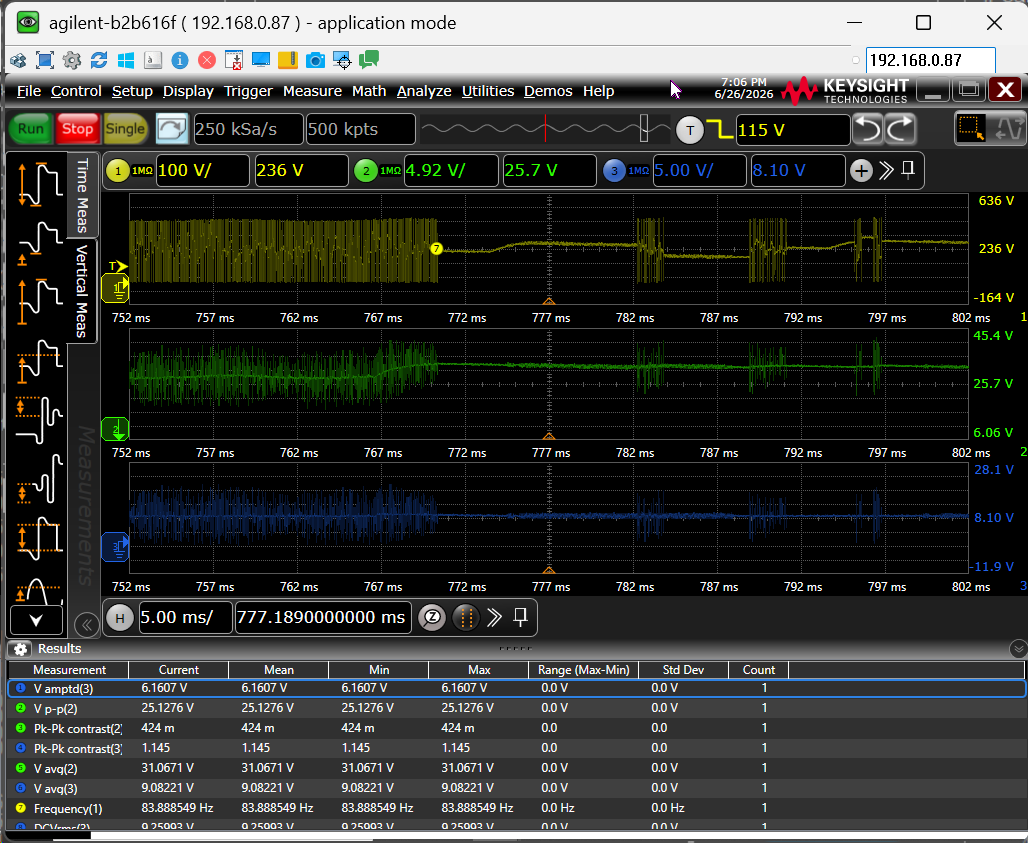
\includegraphics[width=\linewidth]{Data/measurements/evidence/PDO9_3A_to_NoLoad/keysight_9v_3a_to_0a_transient.png}
\caption{\SI{9}{\volt}: \SI{3}{\ampere} to no load.}
\end{subfigure}
\par\medskip
\begin{subfigure}[t]{0.48\textwidth}
\centering
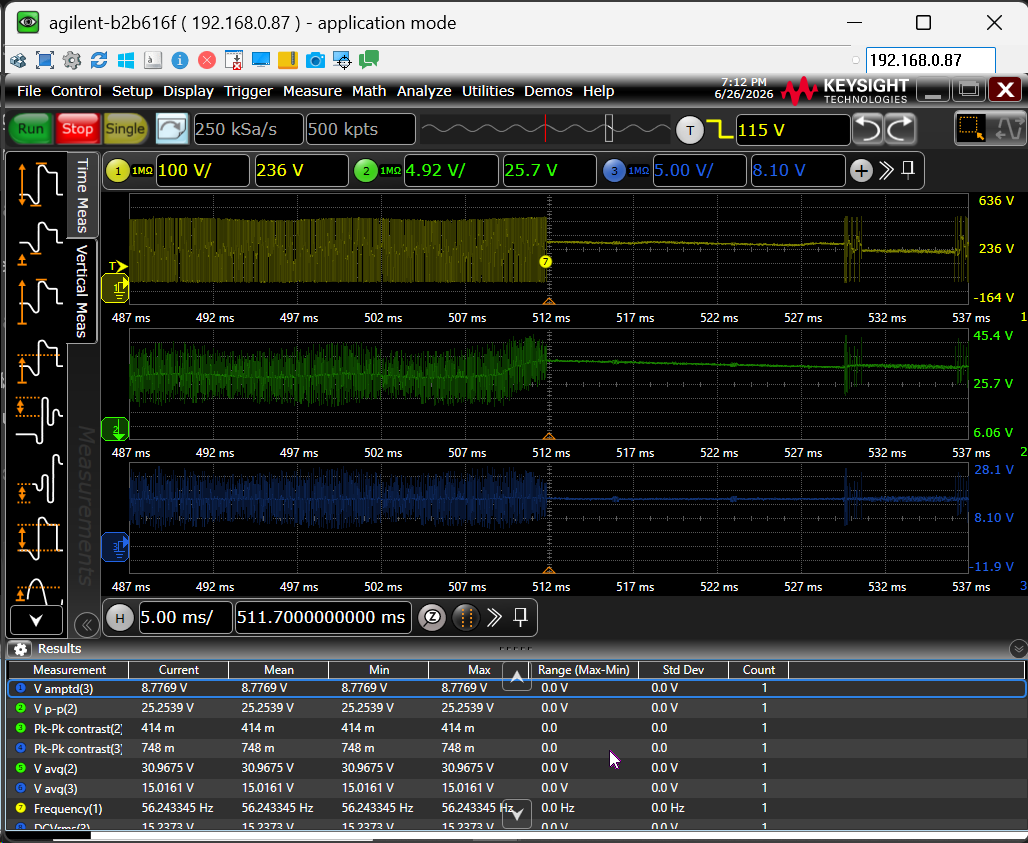
\includegraphics[width=\linewidth]{Data/measurements/evidence/PDO15_3A_TO_NL/keysight_15v_3a_to_0a_transient_sw_secondary_vbus.png}
\caption{\SI{15}{\volt}: \SI{3}{\ampere} to no load.}
\end{subfigure}\hfill
\begin{subfigure}[t]{0.48\textwidth}
\centering
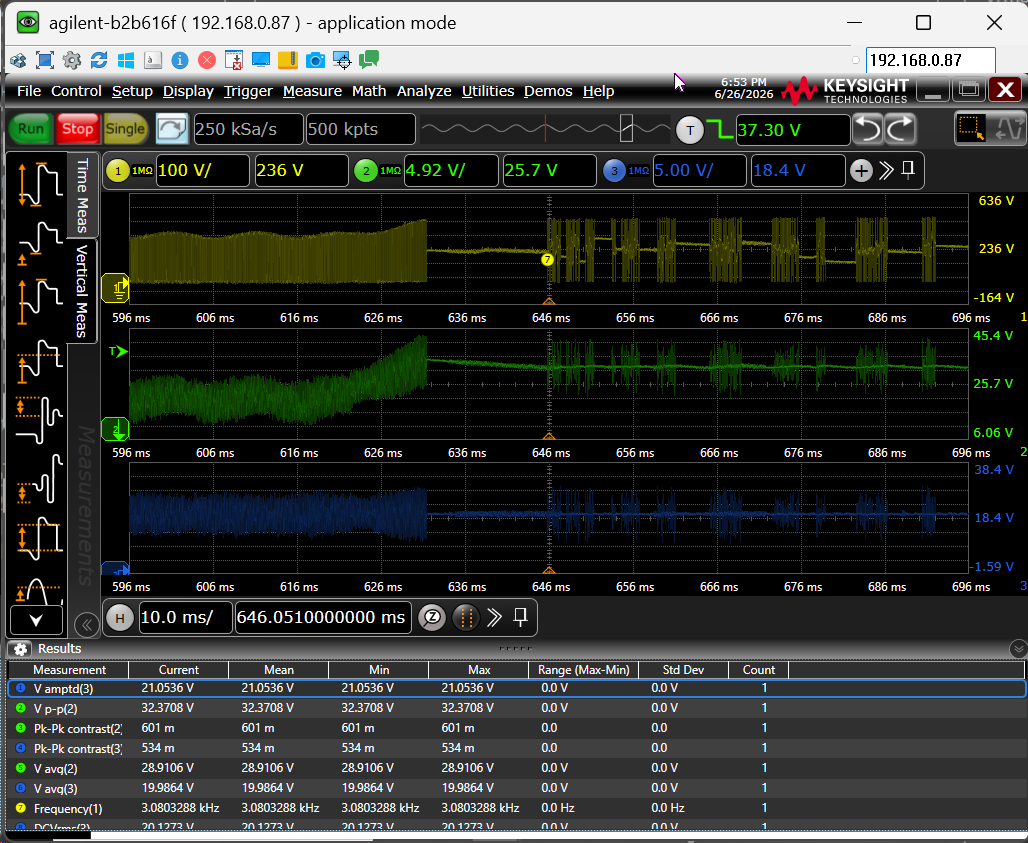
\includegraphics[width=\linewidth]{Data/measurements/evidence/PDO20_80W_to_NoLoad/keysight_80w_to_no_load_secondary_vbus.png}
\caption{\SI{20}{\volt}: nominal \SI{80}{\watt} load removal.}
\end{subfigure}
\caption{Voltage response during load removal. Yellow: half-bridge switch-node voltage. Green: secondary output voltage. Blue: USB-C VBUS output voltage.}
\label{fig:load-transient-scope-evidence}
\label{fig:load-removal-scope-evidence}
\end{figure}

\begin{table}[htbp]
\centering
\caption{Load-removal voltage readings. Average and peak-to-peak values cover the full acquisition and do not give the overshoot from the pre-step voltage.}
\label{tab:load-transient-results}
\small
\begin{tabularx}{\textwidth}{@{}L{0.26\textwidth}L{0.19\textwidth}L{0.16\textwidth}X@{}}
\toprule
Record & Transition & VBUS avg (V) & Logged VBUS pp (V)\\
\midrule
\sourcefile{PDO9-3A-TO-NL-001}, row 31 & \SI{3}{\ampere} to \SI{0}{\ampere} & 9.08221 & 1.145\\
\sourcefile{PDO15-3A-TO-NL-001}, row 35 & \SI{3}{\ampere} to \SI{0}{\ampere} & 15.0161 & 0.414\\
\bottomrule
\end{tabularx}
\end{table}

A numerical overshoot measurement would use
\begin{equation}
\Delta V_\mathrm{over}=V_\mathrm{max}-V_\mathrm{pre},
\end{equation}
using the pre-step mean and a synchronized event marker. Recovery requires
a specified regulation band. Neither result can be calculated from the
acquisition-wide pp readings. Burst-enable PA10 and UART state were not
recorded at the same time, so the response cannot be assigned to
\texttt{LBOOST}, the voltage window, or no-load guarding. Repeated steps
with event markers are needed to measure each response.

\section{Open-Circuit Operation}
\label{sec:res-open}

With the connector unloaded, average VBUS remained close to the selected
output. The DC-coupled means were \SI{5.00727}{\volt},
\SI{9.02697}{\volt}, and \SI{15.0537}{\volt} at the
\SI{5}{\volt}, \SI{9}{\volt}, and \SI{15}{\volt} settings,
respectively. These values were approximately \SI{0.145}{\percent},
\SI{0.300}{\percent}, and \SI{0.358}{\percent} above their targets.

\begin{table}[htbp]
\centering
\caption{No-load voltage readings. The pp column contains the workbook values; the \SI{20}{\volt} entry instead gives AC-coupled statistics.}
\label{tab:open-circuit-results}
\small
\begin{tabularx}{\textwidth}{@{}L{0.28\textwidth}L{0.18\textwidth}L{0.19\textwidth}X@{}}
\toprule
Test & VBUS avg (V) & Logged pp/detail (V) & Capture type\\
\midrule
\sourcefile{PDO5-NL-001} & 5.00727 & 1.396 & DC-coupled\\
\sourcefile{PDO9-NL-001} & 9.02697 & 1.517 & DC-coupled\\
\sourcefile{PDO15-NL-001} & 15.0537 & 1.092 & DC-coupled\\
\sourcefile{PDO20-NL-AC-001} & Unavailable & 0.0762184 & AC detail/statistics\\
\bottomrule
\end{tabularx}
\end{table}

Steady-state no-load input power remains undetermined: the \SI{5}{\volt}
and \SI{9}{\volt} screens include transient or statistical history, and the
\SI{15}{\volt} record lacks settled input power. At \SI{20}{\volt}, AC coupling
also prevents an absolute-output measurement. Unloaded operation and load
removal are described in Section~\ref{sec:res-transient}. Protection margin
is checked by comparing the peak voltage with the active OVP threshold
during the same event.

\section{Switching Waveforms and ZVS}
\label{sec:res-zvs}

The MCU burst-enable pin PA10 groups the nominal \SI{1}{\mega\hertz}
carrier into packets. Figure~\ref{fig:pdo20-high-power-scope} shows the
switch-node and output voltages in the high-power tests. The raw C2
waveforms show burst structure and individual switching transitions.

\begin{figure}[htbp]
\centering
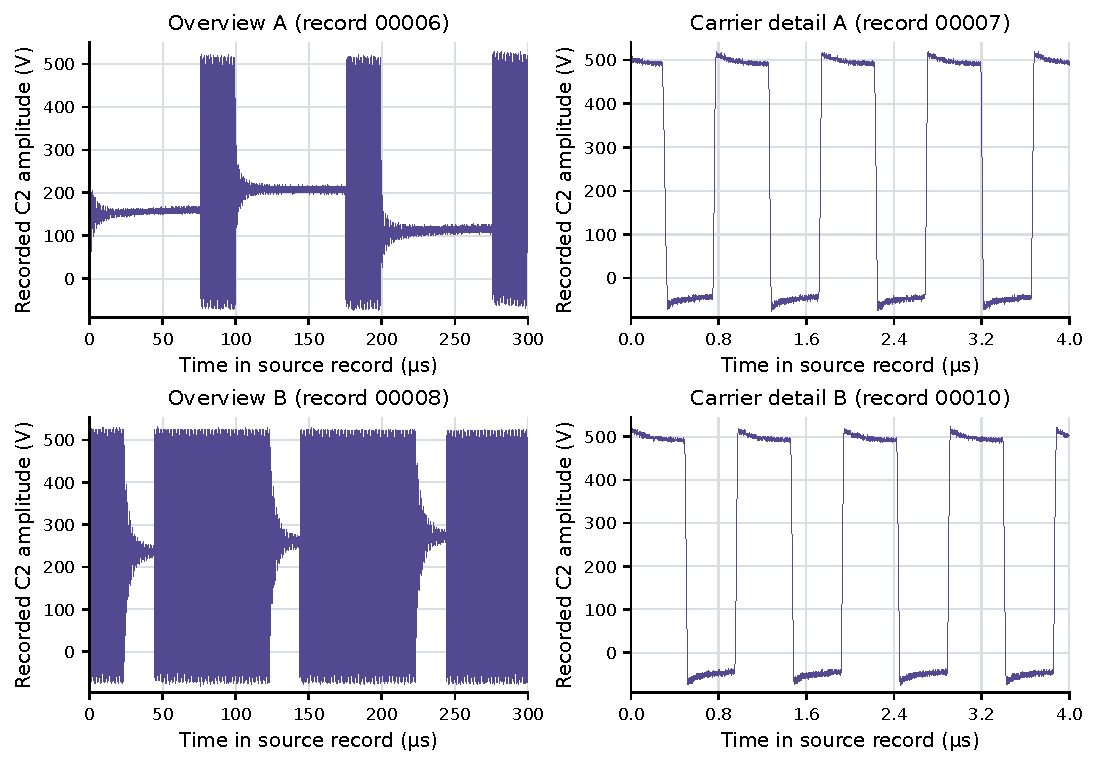
\includegraphics[width=\textwidth]{Pictures/Thesis/10_Results/Rebuilt/raw_switching_records.pdf}
\caption{C2 waveforms showing burst overviews (00006 and 00008) and carrier detail (00007 and 00010).}
\label{fig:switching-waveform-evidence}
\label{fig:rebuilt-raw-switching}
\end{figure}
\FloatBarrier

The overview records show packets followed by ringing toward an intermediate
node voltage. Switching occupies more of the displayed interval in record 00008 than
in record 00006. In the detail views, the median spacing between rising transitions detected
with hysteresis is about \SI{0.967}{\micro\second}, corresponding to
approximately \SI{1.03}{\mega\hertz}. This is the frequency measured in the C2
waveforms; the configured timer frequency and test conditions were not recorded.

The resonant current can discharge half-bridge capacitances before turn-on
\cite{ammar2020chargepump,ammar2021led}. Turn-on voltage is measured
from the incoming device's gate-source transition and drain-source voltage
on the same calibrated time base. The quantity
\begin{equation}
V_\mathrm{DS,res}=V_\mathrm{DS}(t_\mathrm{gate,on})
\end{equation}
has to be evaluated when the gate reaches a stated turn-on threshold.
The single-node captures do not locate that instant.

\begin{table}[htbp]
\centering
\caption{Switching-waveform observations and missing measurements.}
\label{tab:zvs-results}
\begin{tabularx}{\textwidth}{@{}L{0.31\textwidth}X@{}}
\toprule
Capture & Observation or missing measurement\\
\midrule
Main DC-coupled captures & Switching and output-bus behavior at identified loads\\
Raw overview and detail records & Burst structure and approximately \SI{1.03}{\mega\hertz} carrier activity in the exported records\\
Gate-source timing and deskew missing & Residual turn-on voltage and actual dead time cannot be measured from these captures\\
\bottomrule
\end{tabularx}
\end{table}

ZVS remains unverified, particularly at packet boundaries. Classification
requires gate-referenced turn-on captures with known probe loading, return
inductance, deskew, and amplitude calibration.

\section{Input Power Quality}
\label{sec:res-pq}

The high-power \SI{20}{\volt} records gave the best logged input power quality.
Between \SI{3.7}{\ampere} and \SI{4}{\ampere}, PF approached unity and
current THD was lower than at several low-power points
(Figure~\ref{fig:rebuilt-pq}).

\begin{figure}[htbp]
\centering
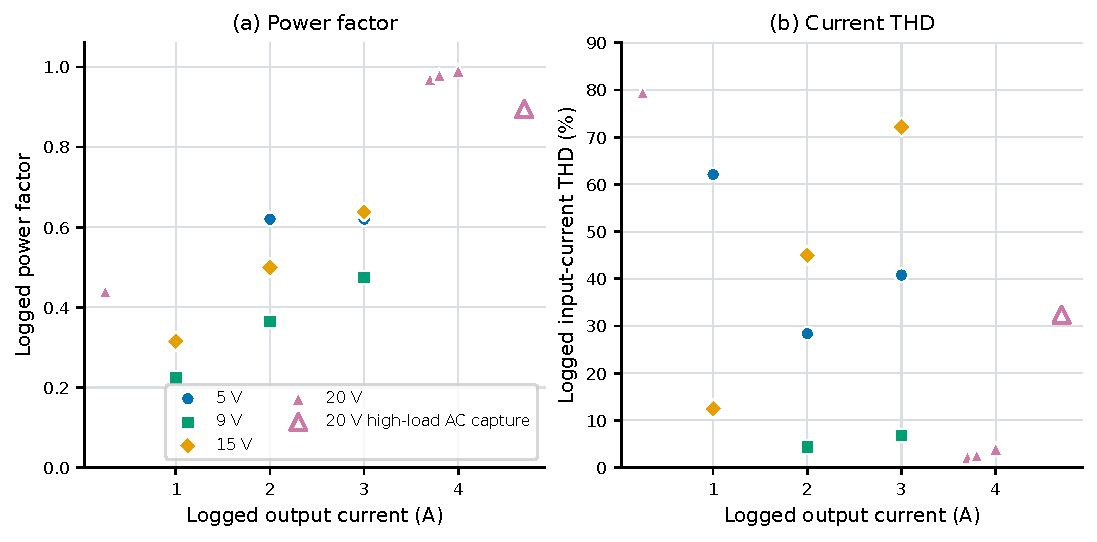
\includegraphics[width=\textwidth]{Pictures/Thesis/10_Results/Rebuilt/power_quality.pdf}
\caption{Measured input PF and current THD versus load. Filled markers use DC-coupled output measurements; the open marker is the \SI{4.7}{\ampere} test with AC-coupled output channels. Some PF and THD readings come from different instruments. Only measured points are shown.}
\label{fig:rebuilt-pq}
\end{figure}

For a common averaging interval, power factor is
\begin{equation}
\mathrm{PF}=\frac{P_\mathrm{in}}{V_\mathrm{in,rms}I_\mathrm{in,rms}},
\end{equation}
and current THD is
\begin{equation}
\mathrm{THD}_I=
\frac{\sqrt{\sum_{n=2}^{N}I_{n,\mathrm{rms}}^2}}
{I_{1,\mathrm{rms}}}\,100\%.
\end{equation}
The logged readings are plotted directly. Some rows combine Siglent PF and
ITECH THD from separate captures. Those readings cannot be used together to
calculate displacement factor.

At \SI{20}{\volt}, the \SI{3.7}{\ampere}, \SI{3.8}{\ampere}, and
\SI{4.0}{\ampere} tests give PF of 0.97, 0.98, and 0.99, with current
THD of \SI{2.23}{\percent}, \SI{2.62}{\percent}, and
\SI{3.98}{\percent}. The \SI{3.9}{\ampere} point was omitted from
the trend because its power-quality entries repeat an associated measurement
set.
The \SI{4.7}{\ampere} capture gives Siglent PF 0.894 and ITECH THD
\SI{32.42}{\percent}, with an earlier firmware revision identified in Table~\ref{tab:prototype-identity}. The
difference includes changed firmware and measurement conditions as well as
load; it cannot be attributed to load alone.

\begin{figure}[htbp]
\centering
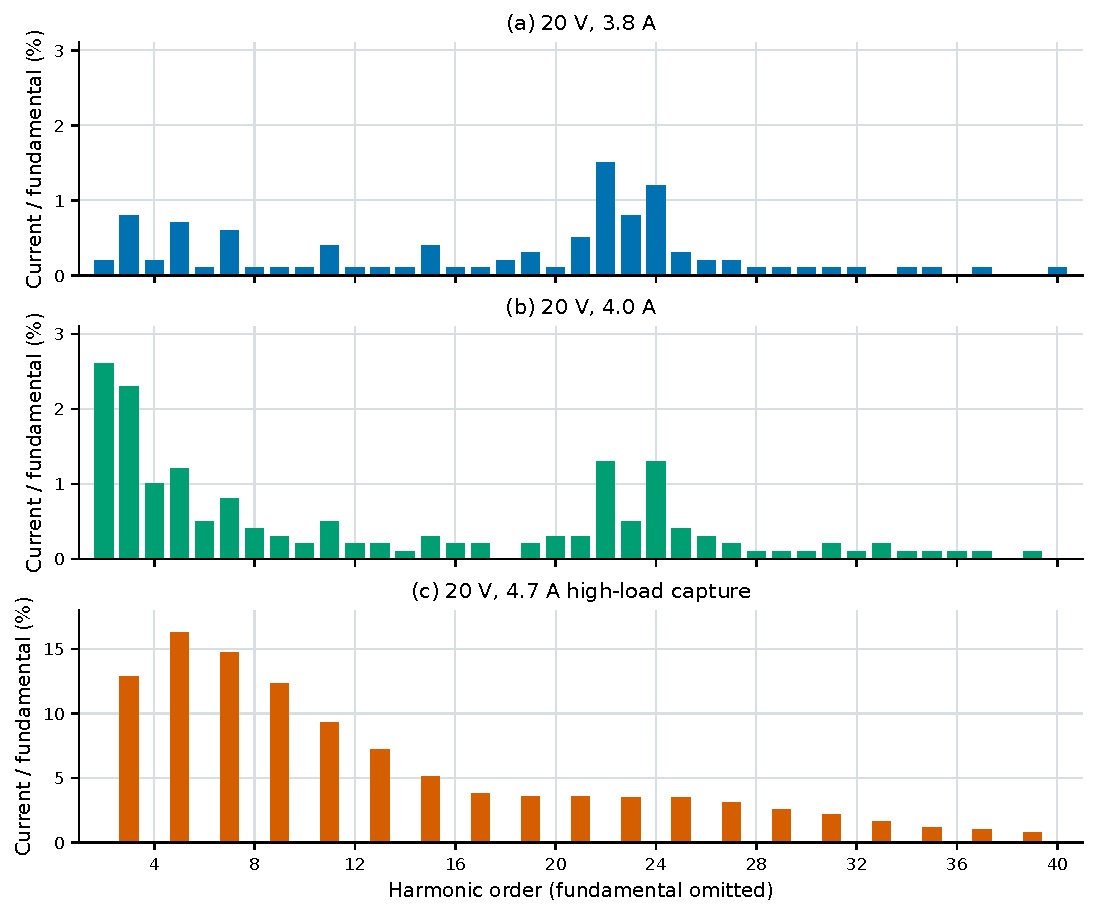
\includegraphics[width=0.96\textwidth]{Pictures/Thesis/10_Results/Rebuilt/current_harmonic_spectrum.pdf}
\caption{Normalized input-current harmonic spectra transcribed from the original ITECH tables at \SI{3.8}{\ampere}, \SI{4.0}{\ampere}, and the \SI{4.7}{\ampere} high-load setting. The fundamental is omitted for readability. The upper panels use a 0--3.1\% scale; the lower panel uses a 0--18\% scale. All orders 1--40 are included in Table~\ref{tab:input-harmonics}.}
\label{fig:rebuilt-harmonic-spectrum}
\end{figure}

At \SI{3.8}{\ampere},
the largest listed component above the fundamental is the 22nd harmonic at
\SI{1.5}{\percent}. At \SI{4.0}{\ampere}, the second and third are
\SI{2.6}{\percent} and \SI{2.3}{\percent}. At \SI{4.7}{\ampere}, the
third, fifth, seventh, and ninth dominate at \SI{12.9}{\percent},
\SI{16.3}{\percent}, \SI{14.7}{\percent}, and \SI{12.3}{\percent}
of the fundamental. Screenshot-checked components through order 40 give
root-sum-square THD values of
approximately \SI{2.64}{\percent}, \SI{4.53}{\percent}, and
\SI{32.49}{\percent}. At \SI{4.0}{\ampere}, the reconstructed result
and separate \SI{3.98}{\percent} screen differ by more than table rounding.
The discrepancy remains unresolved; both values are retained pending a
synchronized repeat.

\begin{figure}[htbp]
\centering
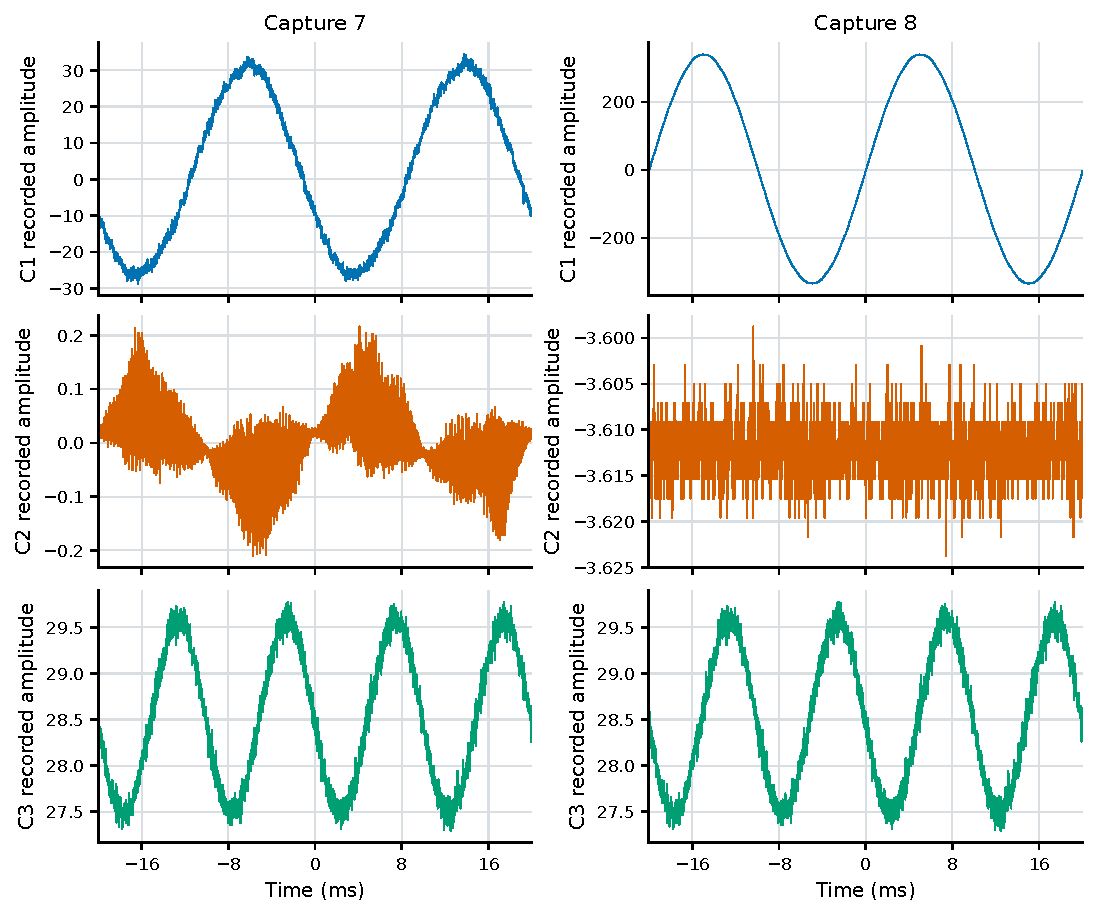
\includegraphics[width=\textwidth]{Pictures/Thesis/10_Results/Rebuilt/raw_line_records.pdf}
\caption{LeCroy line-timescale waveforms from captures 7 and 8. The two C3 records contain identical data.}
\label{fig:rebuilt-raw-line}
\end{figure}

The line-timescale traces show the input waveform, but incomplete probe
calibration prevents calculation of PF or real power from them.

Earlier charge-pump results \cite{ammar2020chargepump,ammar2021led} used
different operating conditions. Input filtering, magnetics, output setting,
and burst structure differ from this prototype. Table~\ref{tab:pq-results} retains the full
readings and identifiers.

\FloatBarrier
\Needspace{14\baselineskip}
\section{Efficiency and Power Difference}
\label{sec:res-efficiency}

Output power, initial efficiency, and input--output power difference
were calculated as
\begin{align}
P_\mathrm{out}&=V_\mathrm{BUS,avg}I_\mathrm{out},
\label{eq:pout-from-vbus-iout}\\
\eta&=\frac{P_\mathrm{out}}{P_\mathrm{in}}\,100\%,
\label{eq:efficiency}\\
P_\mathrm{difference}&=P_\mathrm{in}-P_\mathrm{out}.
\end{align}
Average VBUS and external load current were used to calculate output power,
with analyzer readings for input power. The resulting efficiency estimates
are preliminary because simultaneous acquisition and the inclusion of all
auxiliary power paths are not fully documented.

\begin{figure}[htbp]
\centering
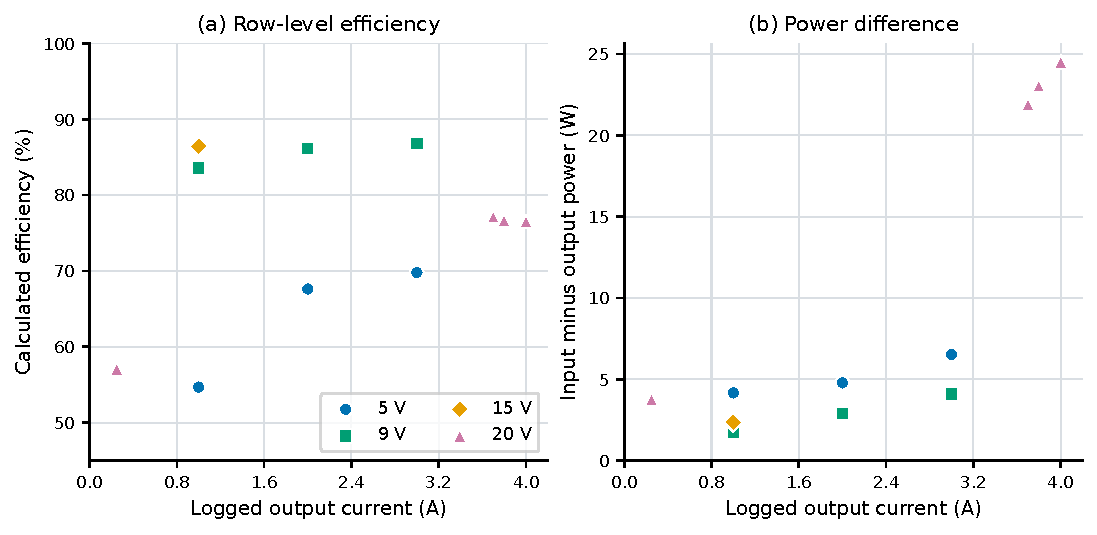
\includegraphics[width=\textwidth]{Pictures/Thesis/10_Results/Rebuilt/efficiency_and_loss.pdf}
\caption{Initial efficiency estimates and input-minus-output power from eleven tests. Marker shapes identify the fixed output voltage. }
\label{fig:rebuilt-efficiency-loss}
\end{figure}

At \SI{5}{\volt}, the calculated value rises from about
\SI{54.7}{\percent} at \SI{1}{\ampere} to \SI{69.8}{\percent} at
\SI{3}{\ampere}. The \SI{9}{\volt} points range from
\SI{83.6}{\percent} to \SI{86.8}{\percent}, the highest of the eleven
selected rows. The \SI{15}{\volt}, \SI{1}{\ampere} result is
\SI{86.4}{\percent}. The tests used different instruments and operating histories, so these
values do not form a calibrated efficiency map.

\Needspace{20\baselineskip}
% Automatically rebuilt from original records by rebuild_results.py.
\begingroup
\scriptsize
\setlength{\tabcolsep}{3pt}
\renewcommand{\arraystretch}{1.12}
\begin{longtable}{@{}L{0.3022\linewidth} L{0.1067\linewidth} L{0.1244\linewidth} L{0.1244\linewidth} L{0.0978\linewidth} L{0.1244\linewidth}@{}}
\caption{Initial efficiency estimates from eleven measurements.}\label{tab:efficiency-results}\\
\toprule
Test ID & $I_\mathrm{out}$ (A) & $P_\mathrm{out}$ (W) & $P_\mathrm{in}$ (W) & $\eta$ (\%) & Difference (W)\\
\midrule
\endfirsthead
\toprule
Test ID & $I_\mathrm{out}$ (A) & $P_\mathrm{out}$ (W) & $P_\mathrm{in}$ (W) & $\eta$ (\%) & Difference (W)\\
\midrule
\endhead
\sourcefile{PDO5-5W-001} & 1.00 & 5.03 & 9.20 & 54.69 & 4.17\\
\sourcefile{PDO5-10W-2A-001} & 2.00 & 9.99 & 14.78 & 67.61 & 4.79\\
\sourcefile{PDO5-MAX3A-001} & 3.00 & 15.06 & 21.59 & 69.79 & 6.52\\
\sourcefile{PDO20-5W-001} & 0.25 & 5.01 & 8.78 & 57.09 & 3.77\\
\sourcefile{PDO20-75W-001} & 3.70 & 73.97 & 95.88 & 77.15 & 21.91\\
\sourcefile{PDO20-76W-38A-001} & 3.80 & 75.93 & 98.99 & 76.70 & 23.06\\
\sourcefile{PDO20-80W-40A-001} & 4.00 & 79.89 & 104.42 & 76.51 & 24.53\\
\sourcefile{PDO9-9W-1A-001} & 1.00 & 9.02 & 10.80 & 83.56 & 1.77\\
\sourcefile{PDO9-18W-2A-001} & 2.00 & 18.03 & 20.93 & 86.14 & 2.90\\
\sourcefile{PDO9-27W-3A-001} & 3.00 & 27.00 & 31.10 & 86.82 & 4.10\\
\sourcefile{PDO15-15W-1A-001} & 1.00 & 15.01 & 17.37 & 86.41 & 2.36\\
\bottomrule
\end{longtable}
\endgroup


The \SI{20}{\volt} high-power tests give \SI{77.15}{\percent},
\SI{76.70}{\percent}, and \SI{76.51}{\percent} at
\SI{3.7}{\ampere}, \SI{3.8}{\ampere}, and \SI{4.0}{\ampere}.
Their input--output differences are \SI{21.91}{\watt},
\SI{23.06}{\watt}, and \SI{24.53}{\watt}. At \SI{4}{\ampere},
\SI{104.418}{\watt} logged input accompanies \SI{79.8928}{\watt}
calculated output. The total difference does not allocate loss among the GaN
stage, inductors, charge pump, output interface, and auxiliary supply;
intermediate-stage power measurements are required.

No-load, transient, and AC-coupled output rows were excluded, along with the
\SI{3.9}{\ampere}, \SI{20}{\volt} row with an associated input capture
and the \SI{15}{\volt}, \SI{2}{\ampere} and \SI{3}{\ampere} rows
whose notes flag real-power disagreement. Siglent/ITECH disagreement remains in several selected groups; the selected
workbook entries are used consistently, but the instrument error remains unresolved.
A matched sweep must synchronize settled input/output readings and account
for auxiliaries, cable drop, temperature, and propagated uncertainty.

\section{Measured Surface Temperatures}
\label{sec:res-thermal}

Heating became more pronounced as load increased in the \SI{9}{\volt}
and \SI{20}{\volt} image groups. The image labeled \SI{20}{\volt},
\SI{4}{\ampere} shows a \SI{90.4}{\celsius} maximum. At the labeled
\SI{20}{\volt}, \SI{4.7}{\ampere} condition, the maximum is
\SI{102.9}{\celsius}, the highest recorded surface reading.

\begin{figure}[htbp]
\centering
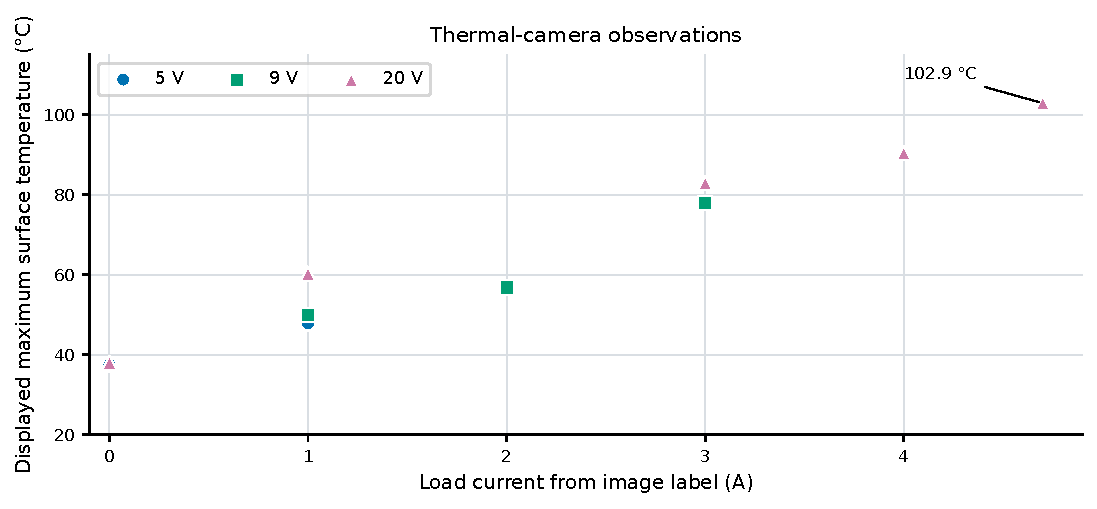
\includegraphics[width=0.95\textwidth]{Pictures/Thesis/10_Results/Rebuilt/thermal_observations.pdf}
\caption{Maximum surface temperatures in the ten thermal images, using the load conditions written on each image. Run duration and airflow were not recorded, so thermal equilibrium cannot be checked.}
\label{fig:rebuilt-thermal}
\end{figure}

The ten no-load and loaded images use an emissivity of 0.95. At
\SI{9}{\volt} and \SI{2}{\ampere}, the camera maximum was
\SI{56.8}{\celsius}, while the cursor read
\SI{39.7}{\celsius}. The plotted temperatures are camera maxima.

\begin{figure}[htbp]
\centering
\begin{subfigure}[t]{0.31\textwidth}
\centering
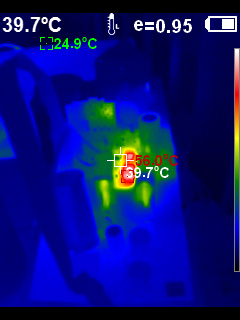
\includegraphics[width=\linewidth,height=0.27\textheight,keepaspectratio]{Pictures/Thesis/10_Results/image_009_9v_2a.png}
\caption{\SI{9}{\volt}, \SI{2}{\ampere}.}
\end{subfigure}\hfill
\begin{subfigure}[t]{0.31\textwidth}
\centering
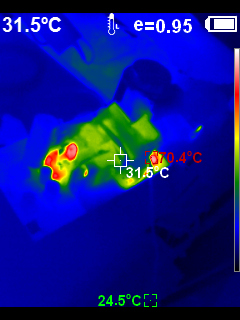
\includegraphics[width=\linewidth,height=0.27\textheight,keepaspectratio]{Pictures/Thesis/10_Results/image_006_20v_4a.png}
\caption{\SI{20}{\volt}, \SI{4}{\ampere}.}
\end{subfigure}\hfill
\begin{subfigure}[t]{0.31\textwidth}
\centering
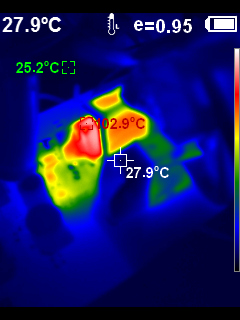
\includegraphics[width=\linewidth,height=0.27\textheight,keepaspectratio]{Pictures/Thesis/10_Results/image_001_20v_4p7a.png}
\caption{\SI{20}{\volt}, \SI{4.7}{\ampere}.}
\end{subfigure}
\caption{Thermal images with their camera readings and test labels.}
\label{fig:thermal-9v-2a-hotspot}
\end{figure}

% Automatically rebuilt from original records by rebuild_results.py.
\begingroup
\scriptsize
\setlength{\tabcolsep}{3pt}
\renewcommand{\arraystretch}{1.12}
\begin{longtable}{@{}L{0.3400\linewidth} L{0.1800\linewidth} L{0.1800\linewidth} L{0.1800\linewidth}@{}}
\caption{Temperature readings from ten thermal images, using emissivity 0.95. The lower reference marker was not confirmed as ambient temperature.}\label{tab:thermal-results}\\
\toprule
Image / condition & Maximum (°C) & Cursor (°C) & Reference (°C)\\
\midrule
\endfirsthead
\toprule
Image / condition & Maximum (°C) & Cursor (°C) & Reference (°C)\\
\midrule
\endhead
Image \#1 / 20 V, 4.7 A & 102.9 & 27.9 & 25.2\\
Image \#2 / 20 V, 1 A & 60.3 & 30.8 & 24.9\\
Image \#3 / 20 V, 3 A & 82.9 & 30.6 & 25.2\\
Image \#4 / 5 V, 1 A & 47.8 & 29.1 & 24.7\\
Image \#5 / 20 V, no load & 38.0 & 29.2 & 25.4\\
Image \#6 / 20 V, 4 A & 90.4 & 31.5 & 24.5\\
Image \#7 / 5 V, open & 37.5 & 34.9 & 25.5\\
Image \#8 / 9 V, 1 A & 49.9 & 29.6 & 25.0\\
Image \#9 / 9 V, 2 A & 56.8 & 39.7 & 24.9\\
Image \#10 / 9 V, 3 A & 78.0 & 32.1 & 25.3\\
\bottomrule
\end{longtable}
\endgroup


Hotspot components are incompletely identified, junction temperatures were
not measured, and lower reference markers are not ambient readings. Missing
duration, airflow, camera distance, and temperature histories prevent a
steady-state thermal comparison. The \SI{4.7}{\ampere} record also lacks DC output
voltage, so output power for the nominal \SI{94}{\watt} point cannot be calculated.

The matched electrical results reach approximately \SIrange{74}{80}{\watt}.
Continuous capability requires a stabilized run with identified hotspots,
controlled ambient/airflow, and device and insulation acceptance limits.

\section{What Changed in the Firmware}
\label{sec:res-fwcompare}

The final controller regulates secondary-bulk voltage through PA1, classifies
load from primary current at PA2, and controls average energy transfer through
the MCU burst-enable pin PA10. Carrier outputs PA8/PA9 retain nominal switching
frequency. Both acquisition timing and feedback interpretation were revised.

\begin{table}[htbp]
\centering
\caption{Firmware changes during development.}
\label{tab:firmware-comparison}
\small
\begin{tabularx}{\textwidth}{@{}L{0.20\textwidth}L{0.33\textwidth}X@{}}
\toprule
Stage & Main change & Role in development\\
\midrule
Manual bring-up & Open-loop or manually commanded PA10 with fixed carrier & Enabled switching for low-energy hardware checks\\
Early closed loop & Blocking acquisition and voltage/current-product experiments & Exposed unsuitable acquisition timing and incorrect interpretation of PA2 as output current\\
DMA voltage control & Circular PA0/PA1/PA2 acquisition and PA1 bang-bang regulation & Removed blocking conversion from the active loop and selected secondary voltage as the feedback variable\\
Final voltage control & Loaded averaged duty, \texttt{LBOOST}, no-load guarding, and optional PA0 duty cap & Controller used in the main identified \SI{5}{\volt} and \SI{20}{\volt} tests\\
\bottomrule
\end{tabularx}
\end{table}

The current-sense pin PA2 measures half-bridge current, so multiplying its current indication by secondary voltage
was not a suitable output-power feedback signal. The product-based control
was replaced by secondary-voltage regulation using PA1, while PA2 was retained
for load classification and diagnostics. Optional feed-forward from the primary-voltage input PA0 can cap
the burst-enable duty requested at PA10 as primary voltage rises.

Loaded and load-removal tests show the response of the combined controller;
the contributions of individual changes were not measured separately. The
requested \texttt{MAXRATE} period is \SI{20}{\micro\second}; the achieved
period and jitter have not been measured.

\section{How the Models Differ from the Prototype}
\label{sec:res-simhw}

The supplied LTspice studies were used to interpret charge-pump and resonant
operation. They do not model the manufactured prototype with its final
inductors, GaN package, PCB parasitics, USB-C interface, and sampled PA10 burst
controller.

\begin{table}[htbp]
\centering
\caption{Comparison of the supplied models with the prototype measurements.}
\label{tab:simulation-hardware}
\begin{tabularx}{\textwidth}{@{}L{0.23\textwidth}L{0.34\textwidth}X@{}}
\toprule
Quantity & Measurements & Model comparison\\
\midrule
Carrier and resonant switching & Oscilloscope captures and raw waveform exports & Shows circuit operation; no numerical match\\
Switch-node ringing & Selected screenshots and raw node records & Qualitative only; layout and probe parasitics are not matched\\
Output regulation and detail & DC records and separate AC-detail captures & Experimental results; no matching final model\\
Input current and harmonics & Logged analyzer entries and transcribed spectra & Experimental results; filter, source impedance, and controller are not matched\\
DC-link ripple & No matched model/measurement pair & No numerical comparison\\
\bottomrule
\end{tabularx}
\end{table}

The prototype results are compared with the requirements at the tested loads.
A predictive model comparison requires measured magnetics, component/layout
parasitics, the implemented controller, and matched input and load.

\section{Requirements Met and Tests Still Needed}
\label{sec:res-compliance}

The four selected USB-C outputs were obtained on V1, and \SI{79.89}{\watt} was calculated at its highest matched DC point. Later V2 tests reached \SI{137.1}{\watt} at the secondary output with voltage droop. The \SI{100}{\watt} continuous target, revised \SI{65}{\watt} minimum, and earlier \SI{75}{\watt} validation criterion still need a stabilized run of defined duration.
Section~\ref{sec:revised-plan-criteria} defines these criteria. The measured behavior is compared with the requirements in
Chapter~\ref{ch:requirements}.

\begin{table}[htbp]
\centering
\caption{Prototype requirements and test results.}
\label{tab:requirements-compliance}
\scriptsize
\begin{tabularx}{\textwidth}{@{}L{0.08\textwidth}L{0.25\textwidth}X L{0.17\textwidth}@{}}
\toprule
ID & Requirement & Measurements or implementation & Status\\
\midrule
FR-01 & Controlled startup & Implemented precharge; no synchronized startup capture & Incomplete\\
FR-02 & Fixed carrier and PA10 control & Firmware signal structure and carrier/burst captures & Implemented and observed\\
FR-03 & PA1 voltage regulation & Loaded operation at the four fixed settings & Met at tested points\\
FR-04 & Reduced no-load energy & No-load voltage records; burst control implemented in firmware & Incomplete\\
FR-05 & Recovery after load changes & Load-removal captures; recovery band and timing missing & Response recorded\\
FR-06 & Latched secondary OVP & Implemented in firmware; no measured trip event & Trip not measured\\
FR-07 & ADC DMA acquisition & Circular ADC DMA in the baseline firmware; live timing logs incomplete & Implemented\\
FR-08 & UART configuration and diagnostics & Commands present in source; complete run logs absent & Implemented\\
\midrule
PR-01 & \SI{100}{\watt} continuous target; revised \SI{65}{\watt} minimum; earlier \SI{75}{\watt} validation criterion & V1 connector: \SI{79.89}{\watt}; V2 secondary: \SI{137.1}{\watt} with droop; V2 tests did not reach thermal equilibrium & Continuous criteria unverified\\
PR-02 & State tested AC input & Logged \SI{240}{\volt}, \SI{50}{\hertz} condition & One input condition tested\\
PR-03 & State tested output modes & \SI{5}{\volt}, \SI{9}{\volt}, \SI{15}{\volt}, and \SI{20}{\volt} loaded records & Met at tested points\\
PR-04 & Report mean, ripple, and transients & Average voltage measured; ripple definitions and transient timing incomplete & Incomplete\\
PR-05 & Maximum no-load voltage and OVP margin & No-load captures without complete peak/threshold pair & Unresolved\\
PR-06 & PF and current THD & Logged analyzer entries and current spectra & Measured; standard compliance not tested\\
PR-07 & Efficiency at defined input/output points & Eleven initial estimates; included supplies and timing remain uncertain & Initial estimate\\
PR-08 & Thermal condition and temperature & V1 images: \SI{90.4}{\celsius} at \SI{4}{\ampere}; V2 secondary region: \SI{98.3}{\celsius}; no thermal equilibrium in V2 tests & Surface observations\\
PR-09 & Link results to configuration & Test identifiers and instrument readings & Setup details incomplete\\
PR-10 & Identify active overload limiter & The component or control action limiting power was not isolated & Unresolved\\
\bottomrule
\end{tabularx}
\end{table}
\FloatBarrier

Average output voltage stayed near the selected level at the tested loads. A rated
operating range still requires synchronized power/ripple measurements,
thermal endurance, transient/protection timing, and gate-referenced switching
captures. USB-PD, safety, harmonic-standard, and EMI qualification remain open.

\section{Bring-Up Problems and Changes}
\label{sec:res-failures}

Bring-up required the circuit, sensing, and firmware to be corrected together.
Blocking ADC reads delayed feedback, the initial PA2 interpretation used the
wrong current for output power, and unloaded operation needed a tighter
energy limit. Those problems shaped the final control structure.

\begin{table}[htbp]
\centering
\caption{Bring-up problems, corrections, and design lessons.}
\label{tab:failure-log}
\small
\begin{tabularx}{\textwidth}{@{}L{0.23\textwidth}L{0.36\textwidth}X@{}}
\toprule
Issue & Corrective action & Resulting lesson\\
\midrule
Blocking feedback acquisition & Adopted circular ADC DMA & Acquisition timing must remain compatible with the live control loop\\
PA2 interpreted as output current & Removed PA2-based output-power control; retained PA1 voltage regulation & Match feedback to the physical quantity used by the controller\\
Irregular no-load pulse structure & Revised minimum-cycle handling and no-load duty logic & Schedule complete carrier cycles and limit residual energy explicitly\\
Energy after load removal & Added no-load guarding, voltage windows, and sag recovery paths & Loaded and unloaded operation require distinct control behavior\\
Ambiguous output detail fields & Kept DC, AC detail, and acquisition statistics separate & A range of average readings is not instantaneous output ripple\\
Disagreeing power instruments & Kept the original readings and calculated initial efficiency estimates & State the measurement boundary and synchronization before interpreting losses\\
High-load temperature rise & Recorded camera maxima and the stated test conditions & Follow component temperatures until they settle at the chosen load\\
\bottomrule
\end{tabularx}
\end{table}
\FloatBarrier

PA1 voltage regulation replaced the incorrect power feedback, while PA2
was retained for load classification. Complete-cycle scheduling addressed
irregular pulses, and no-load guarding limited charging after load removal.
The highest calculated V1.0 output was \SI{79.89}{\watt}; further loading toward
the \SI{100}{\watt} objective requires temperature histories alongside the
electrical readings.

The remaining tests must pair input and output power, capture ripple with
known coupling and bandwidth, follow identified temperatures to stabilization,
and record controller state during load and protection events.

\Needspace{11\baselineskip}
\section{Revised Plan: Results and Remaining Work}
\label{sec:res-revised-plan}

The revised plan sets the next engineering tasks:
\SI{100}{\watt} continuous remains the target, \SI{65}{\watt} continuous
is the minimum, and the previously reported approximately \SI{85}{\watt}
V2 point needs to be repeated before diagnosing the gap and evaluating V3
\cite{projectOctoberPlan}. Section~\ref{sec:revised-plan-criteria} gives
the acceptance criteria used below.

The V1.0 reference test, \sourcefile{PDO20-80W-40A-001}, row 27,
gives \SI{19.9732}{\volt} at \SI{4}{\ampere}, or
\SI{79.8928}{\watt}, with the baseline voltage-control firmware. Repeating the reported \SI{85}{\watt} V2 point requires its original
hardware, firmware, and settings.

Section~\ref{sec:res-v2-testing} reports the V2 tests. An earlier \SI{100}{\watt} constant-power load setting was a setpoint. Later secondary-output measurements reached \SI{137.1}{\watt} with voltage droop, and none of those tests reached thermal equilibrium. A matched repeat of the earlier \SI{85}{\watt} point remains open. Input-bridge and secondary-region heating require further investigation.

\begin{table}[htbp]
\centering
\caption[Progress against the revised plan.]{Progress against the revised project plan and remaining tests.}
\label{tab:revised-plan-results-status}
\scriptsize
\begin{tabularx}{\textwidth}{@{}L{0.07\textwidth}L{0.24\textwidth}Y L{0.23\textwidth}@{}}
\toprule
ID & Planned work & Result & Remaining work\\
\midrule
AP-01 & \SI{100}{\watt} target; \SI{65}{\watt} continuous minimum & V1 connector reached \SI{79.8928}{\watt}; V2 secondary reached \SI{137.1}{\watt} with droop and no thermal equilibrium & Run the supply at the specified loads while following temperatures to stabilization\\
AP-02 & Repeat the reported approximately \SI{85}{\watt} V2 baseline & The plan reports the point; the retained matched dataset reaches approximately \SI{80}{\watt} on the identified older assembly & Original hardware/settings and a repeat test are still needed\\
AP-03 & Explain the power gap and identify the highest repeatable safe output & Earlier secondary-winding heating and limited power increase; later higher-current V2 tests with droop and heating at the input bridge and secondary region; suspected interlayer restriction remains under investigation & Measure individual losses, switching behavior, and the condition that limits further loading\\
AP-04 & Validate supported fixed PDOs and PPS & Electrical results at \SI{5}{\volt}, \SI{9}{\volt}, \SI{15}{\volt}, and \SI{20}{\volt}; qualitative load removal & Negotiation, PPS behavior, defined stability bands, and protection responses need matched tests\\
AP-05 & Defined-duration thermal and reliability assessment & V1 images include \SI{90.4}{\celsius} at the labeled \SI{20}{\volt}, \SI{4}{\ampere} condition; later V2 secondary-region maximum was \SI{98.3}{\celsius} & Temperature histories, stabilization, ambient/airflow, and endurance remain incomplete\\
AP-06 & V3 design and release package & A slimmed edge-card layout was prepared with the USB-PD section removed and secondary rectification retained & Design review, fabrication/assembly checks, and replacement-magnetics tests remain incomplete\\
AP-07 & Compare V2/V3 power density using one volume convention & Approximately \SI{8}{\percent} net volume reduction was estimated for the reduced-function V3 layout & Measure both assemblies using the same included hardware, power, and cooling conditions\\
AP-08 & V3 readiness decision or documented fallback & V1 and V2 supply the operating results; V3 reached a slimmed layout, with new magnetics not installed & A V3 readiness decision and matched power/thermal tests remain open\\
\bottomrule
\end{tabularx}
\end{table}
\FloatBarrier

Continuous rating and revision comparison require an identified baseline
followed by duration, temperature, stress, and dynamic tests against declared
limits. The V3 estimate in \cref{sec:res-v3-design} covers the reduced
layout; comparison of the complete supply includes its external USB-PD stage.
Follow-up methods and controlled changes are given
in Sections~\ref{sec:method-plan-validation} and~\ref{sec:disc-plan-gap}.

\section{V2 Testing and Resonant-Tank Changes}
\label{sec:res-v2-testing}

The original V2 tank showed excessive heating in the approximately
\SI{9.4}{\micro\henry} external series inductor. The inductor was removed
and the resonant capacitance changed to approximately
\SI{1.66}{\nano\farad}, allowing operation with transformer leakage alone.

The measured leakage values in Table~\ref{tab:mag-inherited-measurements}
give an ideal series resonance near \SI{0.96}{\mega\hertz}. The in-circuit
resonance still needs to be measured.

\subsection{Half-Bridge Heating and Dead Time}

After the tank was modified and the software dead time was set to about
\SI{60}{\nano\second}, half-bridge heating decreased. Turn-on voltage
and current measurements are still needed to check ZVS.

\subsection{Secondary Output and Comparison with V1}

During earlier V2 tests, secondary-winding heating and limited power increase were observed near
\SIrange{3.3}{3.6}{\ampere} at the secondary output, and the winding was
suspected to limit further power increase. Output behavior was comparable
to V1. After the tank change, the main heating concern shifted to the
input bridge.

\subsection{Input-Bridge Heating}

Heating persisted around input-bridge diodes D4, D5, D9, and D10 after
diode replacement.

In a test at \SI{240}{\volt} AC, \SI{50}{\hertz}, and a
\SI{100}{\watt} constant-power load setting, output voltage remained steady while bridge
surface temperature rose to approximately \SI{80}{\celsius} within seconds,
then more slowly toward \SI{90}{\celsius}, where testing was stopped.

Figure~\ref{fig:v2-bridge-thermal-observation} shows the bridge heating
during a \SI{95}{\watt} run.

\begin{figure}[htbp]
\centering
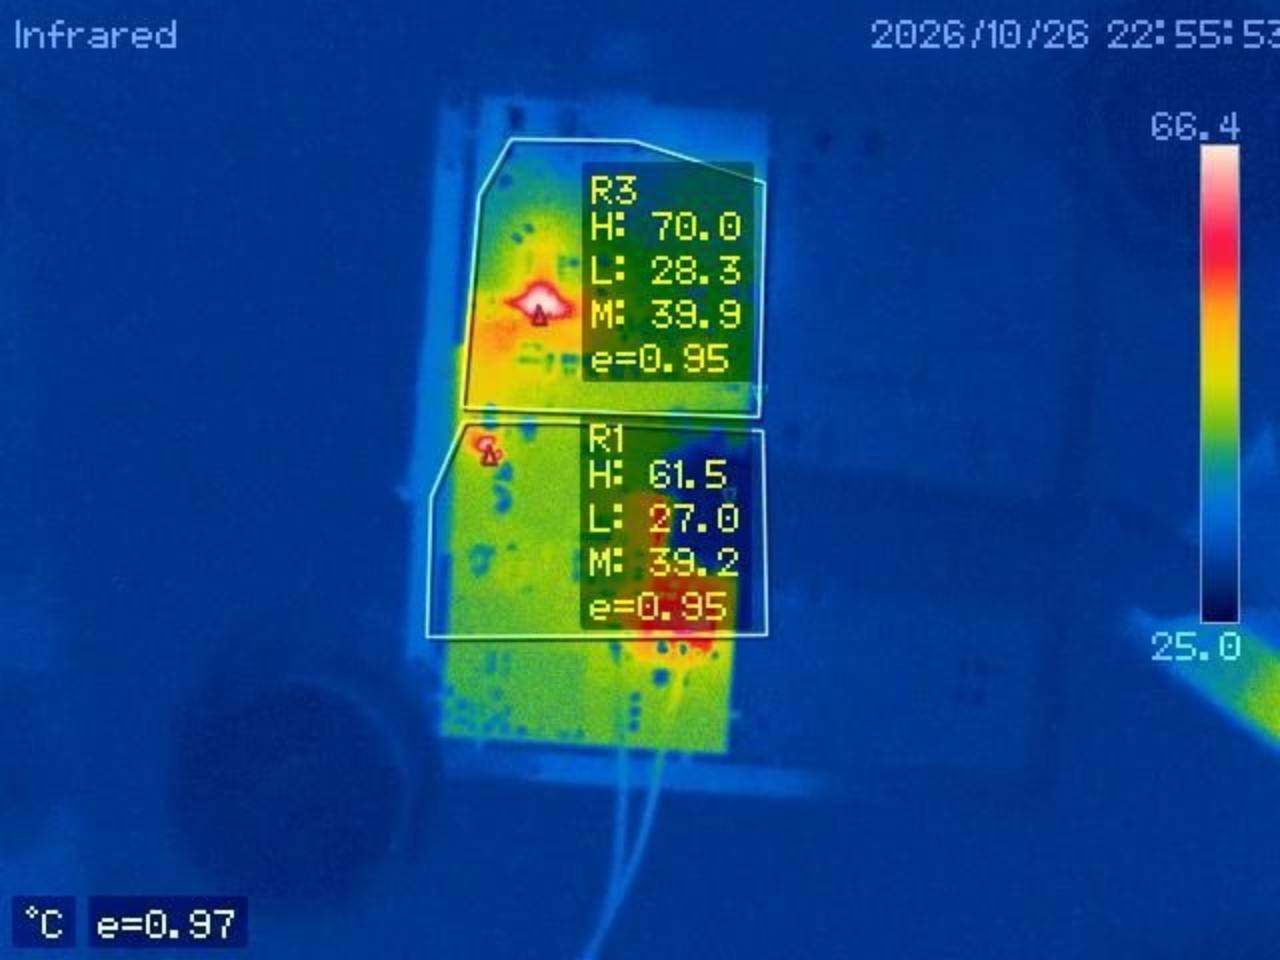
\includegraphics[width=0.80\linewidth]{Data/measurements/v2_results/evidence/v2_bridge_thermal_original.jpg}
\caption{V2 thermal image during the \SI{95}{\watt} run. The displayed surface maxima are \SI{70.0}{\celsius} in R3 and \SI{61.5}{\celsius} in R1.}
\label{fig:v2-bridge-thermal-observation}
\end{figure}
\FloatBarrier

Limited bridge copper and a possible single-via connection between layers
were suspected to contribute to the heating. Narrow current paths add
resistance and restrict heat spreading.

\subsection{Secondary-Output Load and Thermal Tests}
\label{sec:res-v2-secondary-load}

The electronic load was connected to the V2 secondary output. At
approximately \SI{240}{\volt} AC and \SI{50}{\hertz}, increasing the load
current from \SI{1.86}{\ampere} to \SI{10.01}{\ampere} raised the calculated
secondary power from \SI{48.68}{\watt} to \SI{137.08}{\watt}. The secondary
voltage fell from \SI{26.14}{\volt} to \SI{13.69}{\volt} over this sequence
(\cref{tab:v2-secondary-load,fig:v2-secondary-load-performance}). At
\SI{20.07}{\volt}, the load drew \SI{4.29}{\ampere}, giving
\SI{86.17}{\watt}. The higher-power points were therefore reached with
increasing voltage droop.

\begin{table}[htbp]
\centering
\small
\setlength{\tabcolsep}{4pt}
\caption{AC input, secondary-load readings, and thermal-region maxima during the V2 load sequence. Input voltage was approximately \SI{240}{\volt} at \SI{50}{\hertz}.}
\label{tab:v2-secondary-load}
\begin{tabular}{@{}rrrrrrrr@{}}
\toprule
Capture & $P_{\mathrm{in}}$ & $V_{\mathrm{sec}}$ & $I_{\mathrm{sec}}$ & $P_{\mathrm{sec}}$ & $\eta$ & Bridge R3 & Secondary R1\\
 & (W) & (V) & (A) & (W) & (\%) & ($^\circ$C) & ($^\circ$C)\\
\midrule
015 & 64.352 & 26.14 & 1.86 & 48.68 & 75.7 & 65.1 & 50.3\\
017 & 95.142\textsuperscript{*} & 21.36 & 3.31 & 70.75 & 74.4\textsuperscript{*} & 83.9 & 57.2\\
018 & 106.731 & 20.07 & 4.29 & 86.17 & 80.7 & 68.2 & 59.7\\
019 & 121.899 & 18.46 & 5.27 & 97.35 & 79.9 & 73.2 & 69.4\\
020 & 140.565 & 16.87 & 6.51 & 109.87 & 78.2 & 74.5 & 81.6\\
021 & 168.859 & 14.92 & 8.51 & 127.05 & 75.2 & 75.6 & 88.7\\
022 & 189.180 & 13.69 & 10.01 & 137.08 & 72.5 & 73.7 & 98.3\\
\bottomrule
\end{tabular}
\par\vspace{0.4em}
\begin{minipage}{\linewidth}\footnotesize
$P_{\mathrm{sec}}$ is calculated from the electronic-load voltage and current; $\eta=100P_{\mathrm{sec}}/P_{\mathrm{in}}$ is an estimate.
\textsuperscript{*}Capture 017 reports \SI{95.142}{\watt} input, while its \SI{239.99}{\volt} and \SI{0.39}{\ampere} readings give \SI{93.60}{\volt\ampere}. The input reading and associated efficiency need checking.
\end{minipage}
\end{table}


In the thermal images in \cref{fig:v2-secondary-load-thermal}, the input-bridge
region R3 reached \SI{83.9}{\celsius} near
\SI{70.75}{\watt}. Its maxima at the subsequent higher-power points were
lower, between \SI{68.2}{\celsius} and \SI{75.6}{\celsius}. The secondary
region R1 became progressively hotter, rising from \SI{50.3}{\celsius} to
\SI{98.3}{\celsius}.

None of the load points reached thermal equilibrium. The sequence includes
both load changes and continued heating, so the temperatures cannot be
treated as settled values for each power level. Diode selection and the
current and thermal paths around the rectifiers require further work.
The tests show that the leakage-only stage can transfer more than
\SI{100}{\watt} to a secondary load, although voltage droop and continued
heating remain.

\begin{figure}[htbp]
\centering
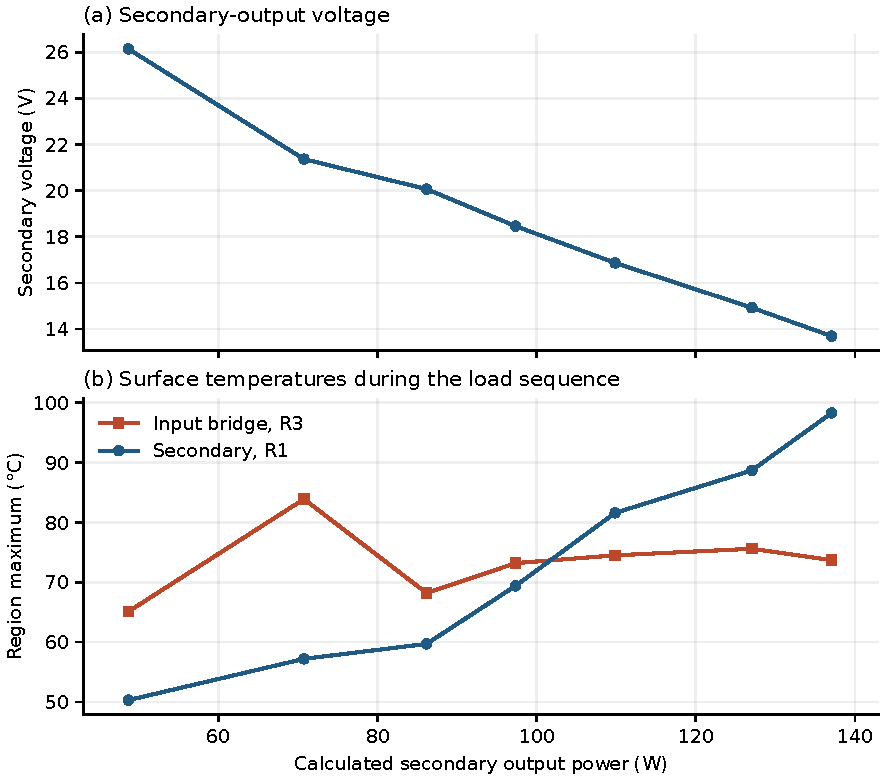
\includegraphics[width=\linewidth]{Data/measurements/v2_load_thermal/load_performance.pdf}
\caption{Secondary voltage and thermal-region maxima during the increasing-load sequence. Lines connect successive readings. R3 covers the input bridge and R1 the secondary area.}
\label{fig:v2-secondary-load-performance}
\end{figure}
\FloatBarrier

\begin{figure}[p]
\centering
\begin{subfigure}{0.78\linewidth}
\centering
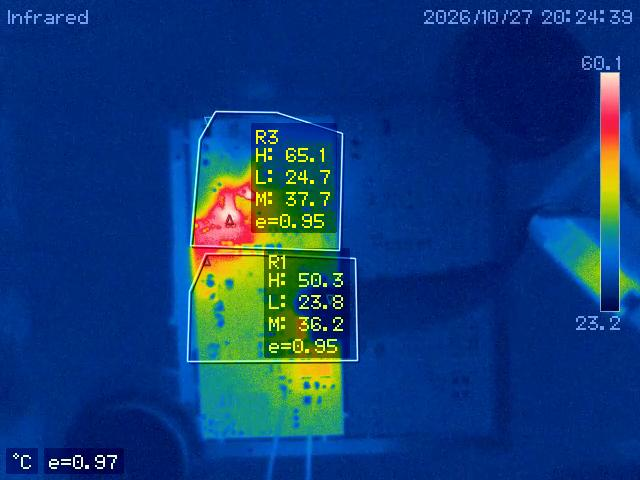
\includegraphics[width=\linewidth]{Data/measurements/v2_load_thermal/thermal/Capture 015-thermal.jpg}
\caption{Capture 015: \SI{48.68}{\watt} at the secondary load.}
\end{subfigure}
\par\vspace{0.8em}
\begin{subfigure}{0.78\linewidth}
\centering
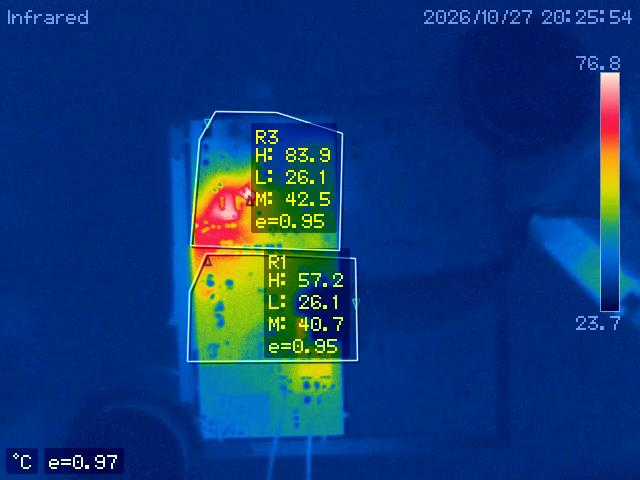
\includegraphics[width=\linewidth]{Data/measurements/v2_load_thermal/thermal/Capture 017-thermal.jpg}
\caption{Capture 017: \SI{70.75}{\watt} at the secondary load.}
\end{subfigure}
\par\vspace{0.8em}
\caption{V2 thermal images during secondary-output loading. R3 covers the input bridge and R1 the secondary area.}
\label{fig:v2-secondary-load-thermal}
\end{figure}
\begin{figure}[p]
\centering
\ContinuedFloat
\begin{subfigure}{0.78\linewidth}
\centering
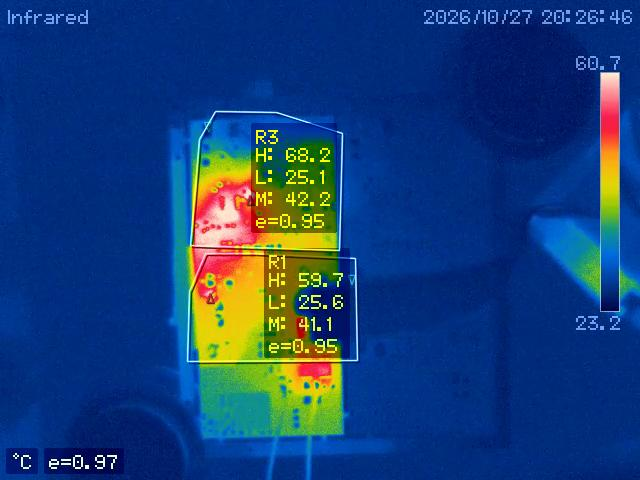
\includegraphics[width=\linewidth]{Data/measurements/v2_load_thermal/thermal/Capture 018-thermal.jpg}
\caption{Capture 018: \SI{86.17}{\watt} at the secondary load.}
\end{subfigure}
\par\vspace{0.8em}
\begin{subfigure}{0.78\linewidth}
\centering
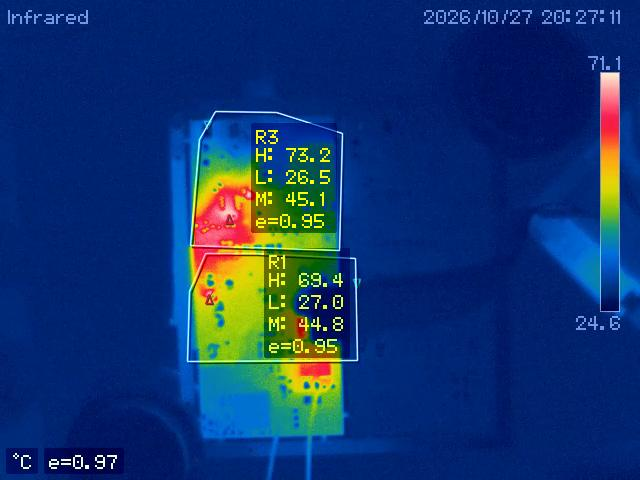
\includegraphics[width=\linewidth]{Data/measurements/v2_load_thermal/thermal/Capture 019-thermal.jpg}
\caption{Capture 019: \SI{97.35}{\watt} at the secondary load.}
\end{subfigure}
\par\vspace{0.8em}
\caption{V2 thermal images during secondary-output loading (continued). R3 covers the input bridge and R1 the secondary area.}
\end{figure}
\begin{figure}[p]
\centering
\ContinuedFloat
\begin{subfigure}{0.78\linewidth}
\centering
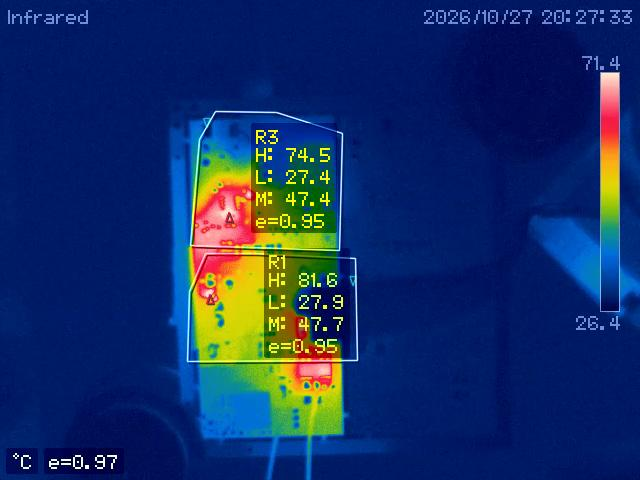
\includegraphics[width=\linewidth]{Data/measurements/v2_load_thermal/thermal/Capture 020-thermal.jpg}
\caption{Capture 020: \SI{109.87}{\watt} at the secondary load.}
\end{subfigure}
\par\vspace{0.8em}
\begin{subfigure}{0.78\linewidth}
\centering
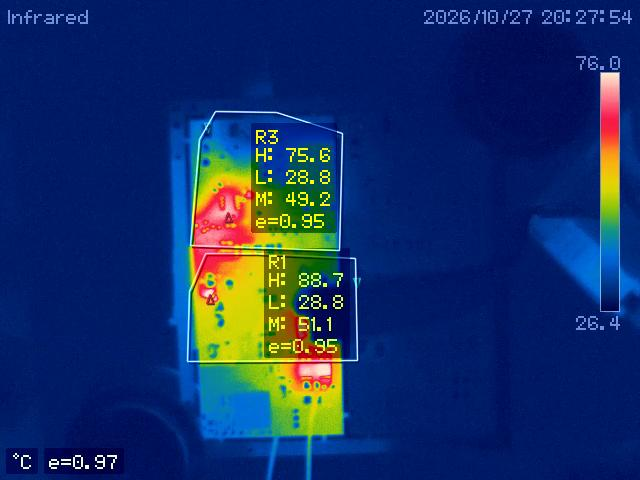
\includegraphics[width=\linewidth]{Data/measurements/v2_load_thermal/thermal/Capture 021-thermal.jpg}
\caption{Capture 021: \SI{127.05}{\watt} at the secondary load.}
\end{subfigure}
\par\vspace{0.8em}
\caption{V2 thermal images during secondary-output loading (continued). R3 covers the input bridge and R1 the secondary area.}
\end{figure}
\begin{figure}[p]
\centering
\ContinuedFloat
\begin{subfigure}{0.78\linewidth}
\centering
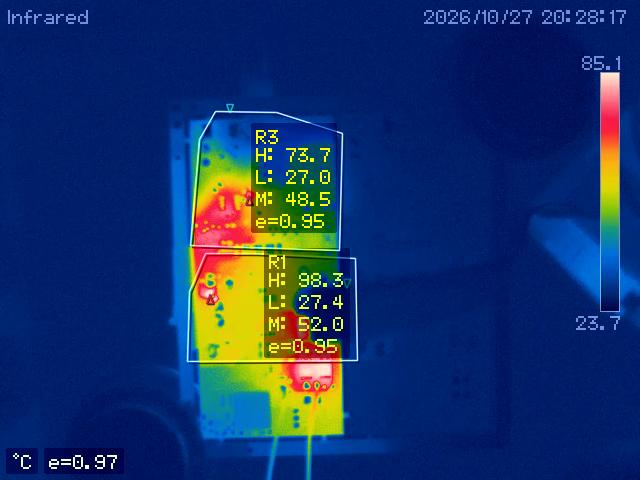
\includegraphics[width=\linewidth]{Data/measurements/v2_load_thermal/thermal/Capture 022-thermal.jpg}
\caption{Capture 022: \SI{137.08}{\watt} at the secondary load.}
\end{subfigure}
\par\vspace{0.8em}
\caption{V2 thermal images during secondary-output loading (continued). R3 covers the input bridge and R1 the secondary area.}
\end{figure}
\FloatBarrier



\subsection{Next Layout Changes}

Wider current paths and more heat-spreading copper are planned for the next
layout. Moving the rectifiers is also being considered to reduce local
heating.


\subsection{V2 Board and Test-Setup Photographs}

The V2 board and thermal-camera setup are shown in
Figure~\ref{fig:v2-board-test-photos}.

\begin{figure}[p]
\centering
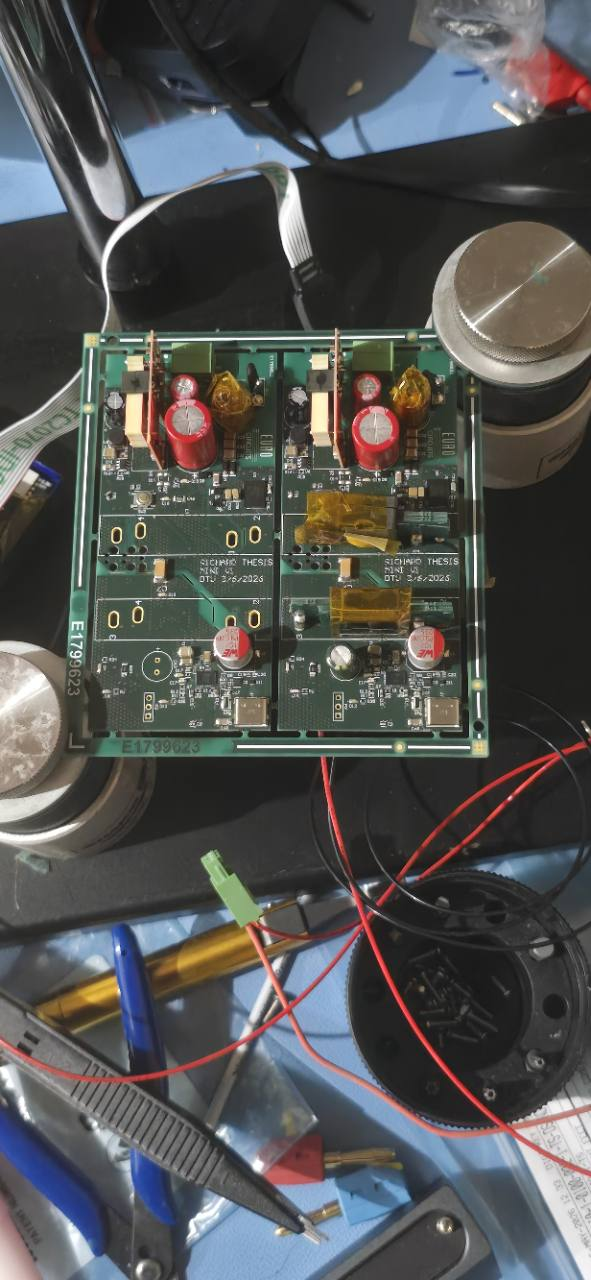
\includegraphics[height=0.34\textheight]{Data/measurements/v2_results/evidence/v2_board_overview_original.jpg}
\hspace{0.03\linewidth}
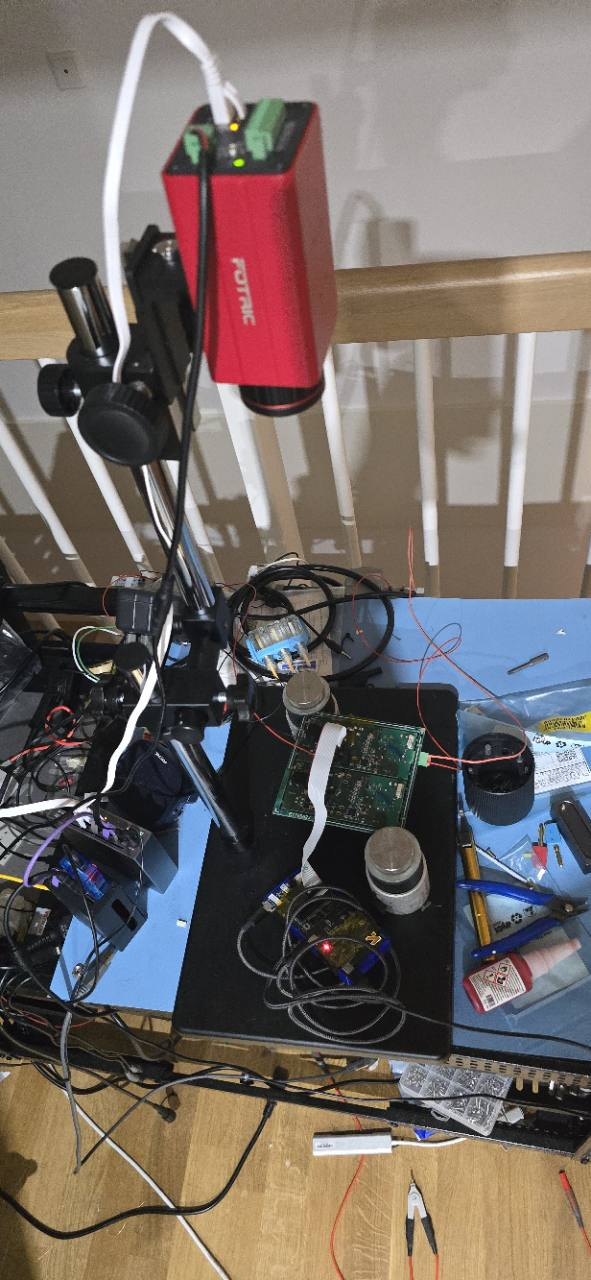
\includegraphics[height=0.34\textheight]{Data/measurements/v2_results/evidence/v2_thermal_setup_original.jpg}

\vspace{0.8em}
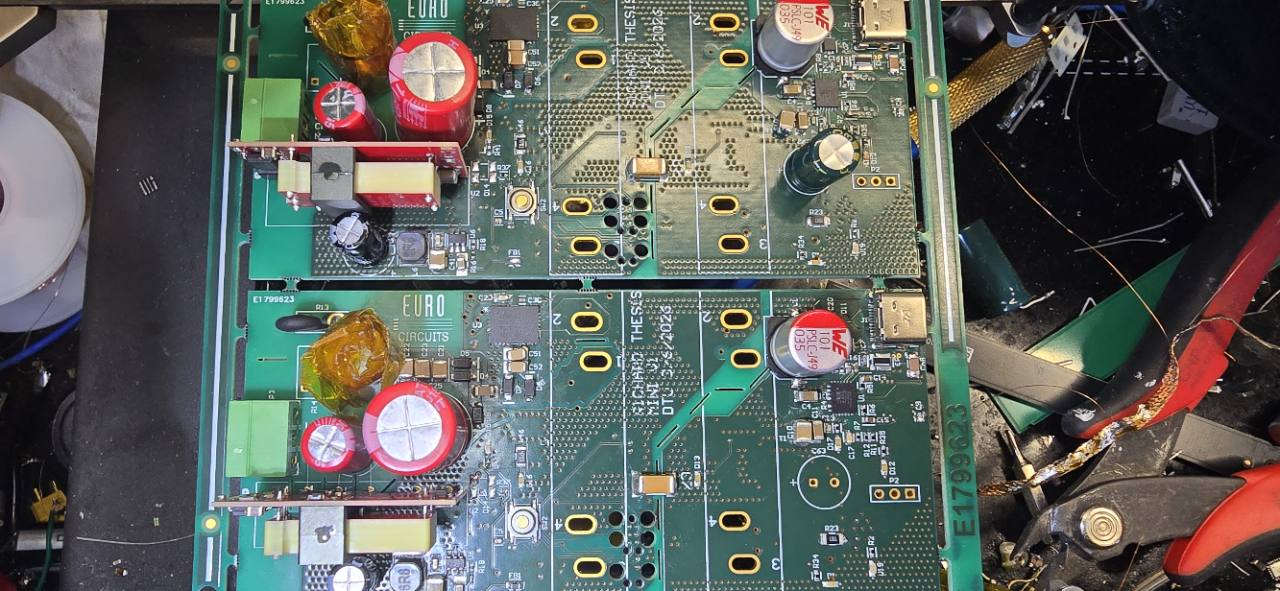
\includegraphics[width=0.86\linewidth]{Data/measurements/v2_results/evidence/v2_board_detail_original.jpg}
\caption{V2 assembly overview (upper left), thermal-camera setup (upper right), and component-side detail (lower).}
\label{fig:v2-board-test-photos}
\end{figure}
\FloatBarrier

\section{V3 Design Outcome and Revision Comparison}
\label{sec:res-v3-design}

The V3 edge-card layout retained secondary rectification and removed the
USB-PD section, giving an estimated net volume reduction of approximately
\SI{8}{\percent}. External regulation and USB-PD remain necessary for a
complete USB-C supply. Replacement planar magnetics were not installed,
and the smaller layout still needs to be built and tested.

\begin{table}[htbp]
\centering
\small
\caption{Main changes and results for each prototype.}
\label{tab:revision-development-outcomes}
\begin{tabularx}{\textwidth}{@{}L{0.14\textwidth}L{0.34\textwidth}Y@{}}
\toprule
Revision & Main change & Result and remaining work\\
\midrule
V1.0/G071 & Converter integration and DMA-based burst control with the downstream USB-C stage & Matched electrical measurements and load-event records; thermal and loss limitations remained\\
V2/F410 & Integrated controller, browser interface, and leakage-only tank trial & Secondary-load tests reached \SI{137.1}{\watt} with voltage droop; input-bridge and secondary heating remained\\
V3 edge card & Slimmed layout with USB-PD section removed and secondary rectification retained & Approximately \SI{8}{\percent} estimated net volume reduction; replacement magnetics and matched power/thermal validation remained incomplete\\
\bottomrule
\end{tabularx}
\end{table}
\FloatBarrier

The winding and input-path observations identify priorities for the next
prototype.
A V2--V3 comparison must match continuous power and thermal conditions and
include all output hardware required for the same function, following
\cref{sec:method-density}.

